\documentclass{article}

% Language setting
% Replace `english' with e.g. `spanish' to change the document language
\usepackage[english]{babel}

% Set page size and margins
% Replace `letterpaper' with `a4paper' for UK/EU standard size
\usepackage[a4paper,top=2cm,bottom=2cm,left=2cm,right=2cm,marginparwidth=2cm]{geometry}

% Useful packages
\usepackage{amsmath}
\usepackage{graphicx}
\usepackage[colorlinks=true, allcolors=black]{hyperref}
\usepackage{bm}
\usepackage{float}  
\usepackage[utf8]{inputenc}
\usepackage{cite}

\usepackage{siunitx}
\usepackage{booktabs}
\usepackage{lipsum}%% a garbage package you don't need except to create examples.
\usepackage{fancyhdr}
\pagestyle{fancy}
\lhead{Wednesday Group A}
\rhead{Line Following Robot}

\renewcommand{\headrulewidth}{0.4pt}
\renewcommand{\footrulewidth}{0.4pt}




\title{%
  \textbf{Line Following Robot} \\
  \large{ENMT221-24S2} \\}
\author{Sarah Tran \\Blake Tolmie \\George Adams \\Michelle Wang }


\begin{document}
\begin{figure}
\centering

\includegraphics[width=0.4\linewidth]{REPORT/uclogov3.jpeg}
\end{figure}



\maketitle
\newpage
\begin{abstract}
This report presents the design, development, and performance analysis of a Line Following Robot (LFR), created as part of the ENMT221-24S2 term 4 project. The goal was to design a robot capable of autonomously navigating a course, following a black line on a white background, under strict design and time constraints. The process involved circuit and PCB design, mechanical prototyping, and microcontroller programming. Challenges encountered during the project included sensor board issues, requiring multiple adjustments and iterative design refinements. The final design demonstrated competitive performance, completing the course in 14.939 seconds and coming in $8^{th}$ place out of 36 teams. Despite successful results, further improvements in sensor integration and control algorithms, such as transitioning to PID control, are suggested to enhance the robot's tracking accuracy and speed. This project provided valuable hands-on experience with real-world testing, electronic design, and mechanical assembly.


\end{abstract}
\newpage
\tableofcontents
\newpage

\section{Introduction}

Automation is becoming increasingly prevalent in modern technology, especially with the rise of artificial intelligence and high labour costs. As mechatronics engineering students, it is important to have a strong understanding of the concepts surrounding this. For the term 4 project, we were tasked to design a line-following robot (commonly abbreviated as ‘LFR’) under the given constraints and limitations as specified by the project brief \cite{enmt221_lfr2024}. This process involves circuit design, PCB layout and manufacturing, mechanical design, and microcontroller programming. The aim was to design a robot that completes the provided course (black line on white background) in under 30 seconds. Line following robots have some real-world applications, such as the transportation of medical equipment in large hospitals \cite{kumaresan2017line}, and autonomous public transport \cite{gumus2016line}.  

\section{Methodology}
\subsection{Circuit Design}
Early in the design process, it was decided that the circuit would be split into a main PCB board and five separate sensor boards. This allowed the sensors to be moved during the mechanical design process, and the distance between them and the ground to be optimised through testing. The design process was split into smaller tasks and delegated to separate teammates. These tasks included motor drivers (Figure \ref{fig:MotorControlCircuit}), power regulation (Figure \ref{fig:VoltageinandReg}), sensors (Figure \ref{fig:SensorSchem}), programming interface and external oscillator (Figure \ref{fig:Crystal}), the microcontroller (Figure \ref{fig:Microcontroller}), and buttons \& LEDs (Figure \ref{fig:RSET}, \ref{fig:led}, and \ref{fig:Motor ON}).
\\

As collaboration was necessary, a major consideration of the design process was the use of the 'labels' function in KiCad, which can link two parts of a schematic together with an invisible virtual wire, to ensure smooth compatibility between systems. Another consideration was the restriction on allowed components (Appendix C), put in place to ensure fairness among teams.


\begin{figure}[H]
    \centering
    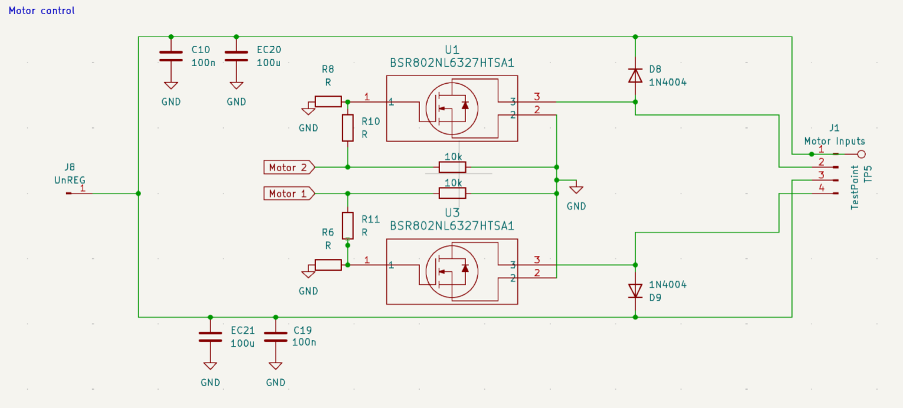
\includegraphics[width=0.8\linewidth]{REPORT/MotorControlCircuit.png}
    \caption{Motor Control Circuit}
    \label{fig:MotorControlCircuit}
\end{figure}

As seen in Figure \ref{fig:MotorControlCircuit}, the motors are controlled by MOSFETs which restrict and allow the flow of power from the unregulated power source through the motors to ground, depending on the input from Motor 1 and 2. These symbols are connected directly to an output capable pin of the microcontroller. As the motors are connected directly to the unregulated power source, capacitors C10, C19, EC20, EC21 are used to filter out unwanted high and low frequencies from the battery source. This use of capacitors is called decoupling. (Note here that C stands for ceramic capacitor which have high capacitance values, while EC stands for electrolytic capacitor which have small values). The motors interface with the circuit through connector J1. Pins 1 and 3 connect directly to the unregulated power source, and to the positive terminals of the motors when assembled. Pins 2 and 4 go to the source pin of the MOSFET and connect to the negative terminals of the motor. As the drain of the MOSFET is connected to ground, when a 3.3V signal comes from the pins of the microcontroller, the unregulated voltage will have a path through the motors to ground, enabling current flow. Flyback diodes D8 and D9 are connected from the MOSFET source pin to the unregulated voltage line, providing a path for back EMF of the motors to cycle through the motor, eventually reducing to 0V and protecting the rest of the circuit from unwanted voltage. 
\\

\begin{figure}[H]
    \centering
    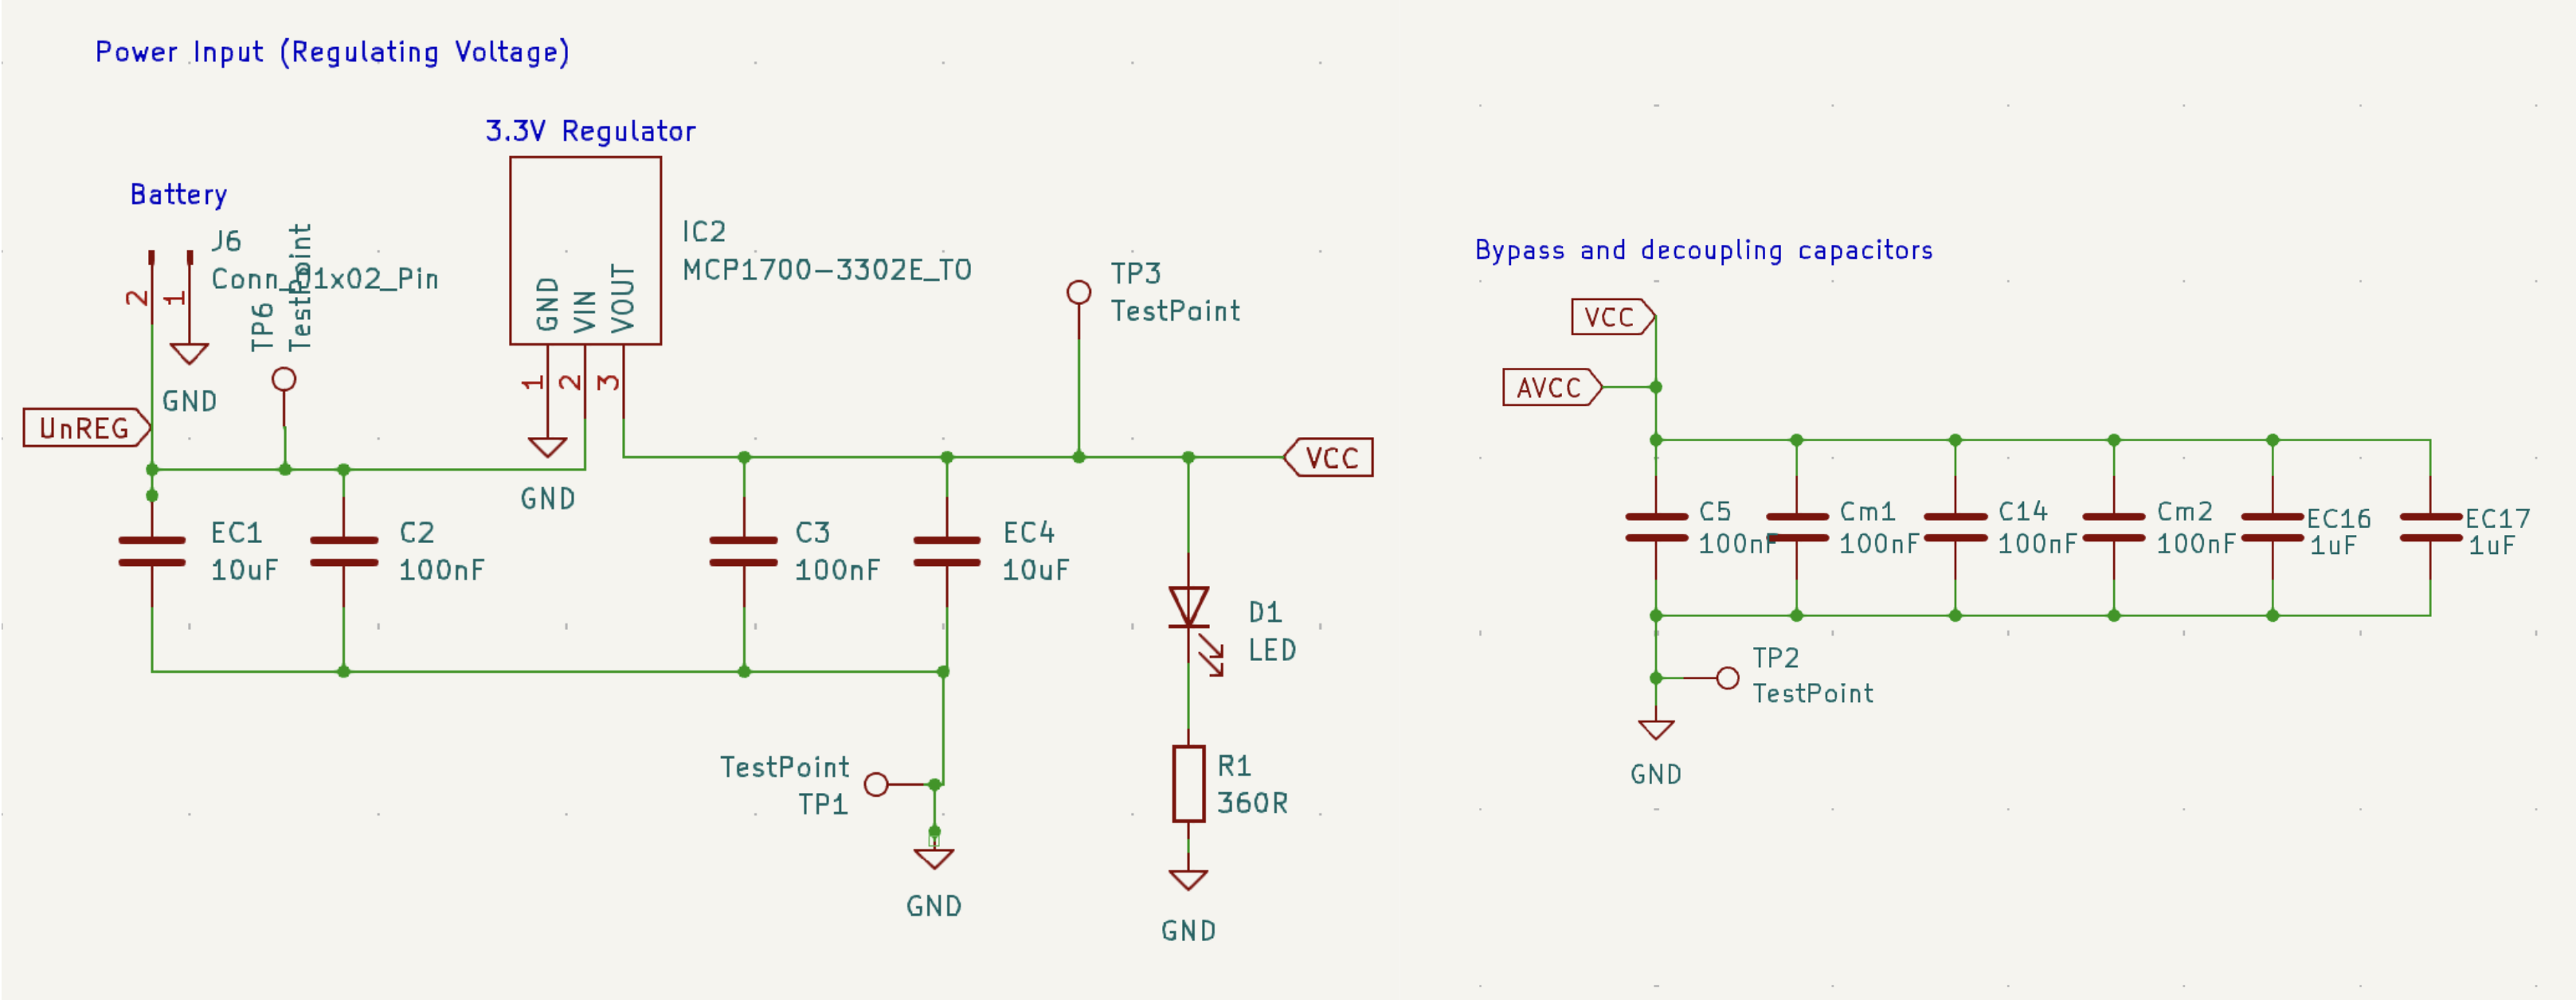
\includegraphics[width=0.8\linewidth]{REPORT/VinputandReg.png}
    \caption{Voltage input and regulation}
    \label{fig:VoltageinandReg}
\end{figure}

Figure \ref{fig:VoltageinandReg} shows how power comes into the circuit. A pack holding four AA batteries was connected to connector J6 labelled ‘Battery’. This was expected to output ~5.5 volts with some fluctuation. This was too high for safe operation of the microcontroller, and with sensitive components such as sensors, we needed some way of reducing the voltage to a manageable level and smoothing it out. The other pin of the battery pack is connected to common ground. After leaving the motor, the unregulated voltage is filtered through decoupling capacitors EC1 and C2 before entering the voltage regulator, IC2. This component outputs VOUT which connects through more decoupling capacitors, C3 and EC4, to the label VCC which is used throughout the circuit as the main power source. Between VCC and ground is a green LED which is used as a ‘power light’ as an easy way to check if the power source is operating correctly. Additionally, there are two test points for unregulated and regulated voltage to help with debugging and circuit analysis. 
\\


\begin{figure}[H]
    \centering
    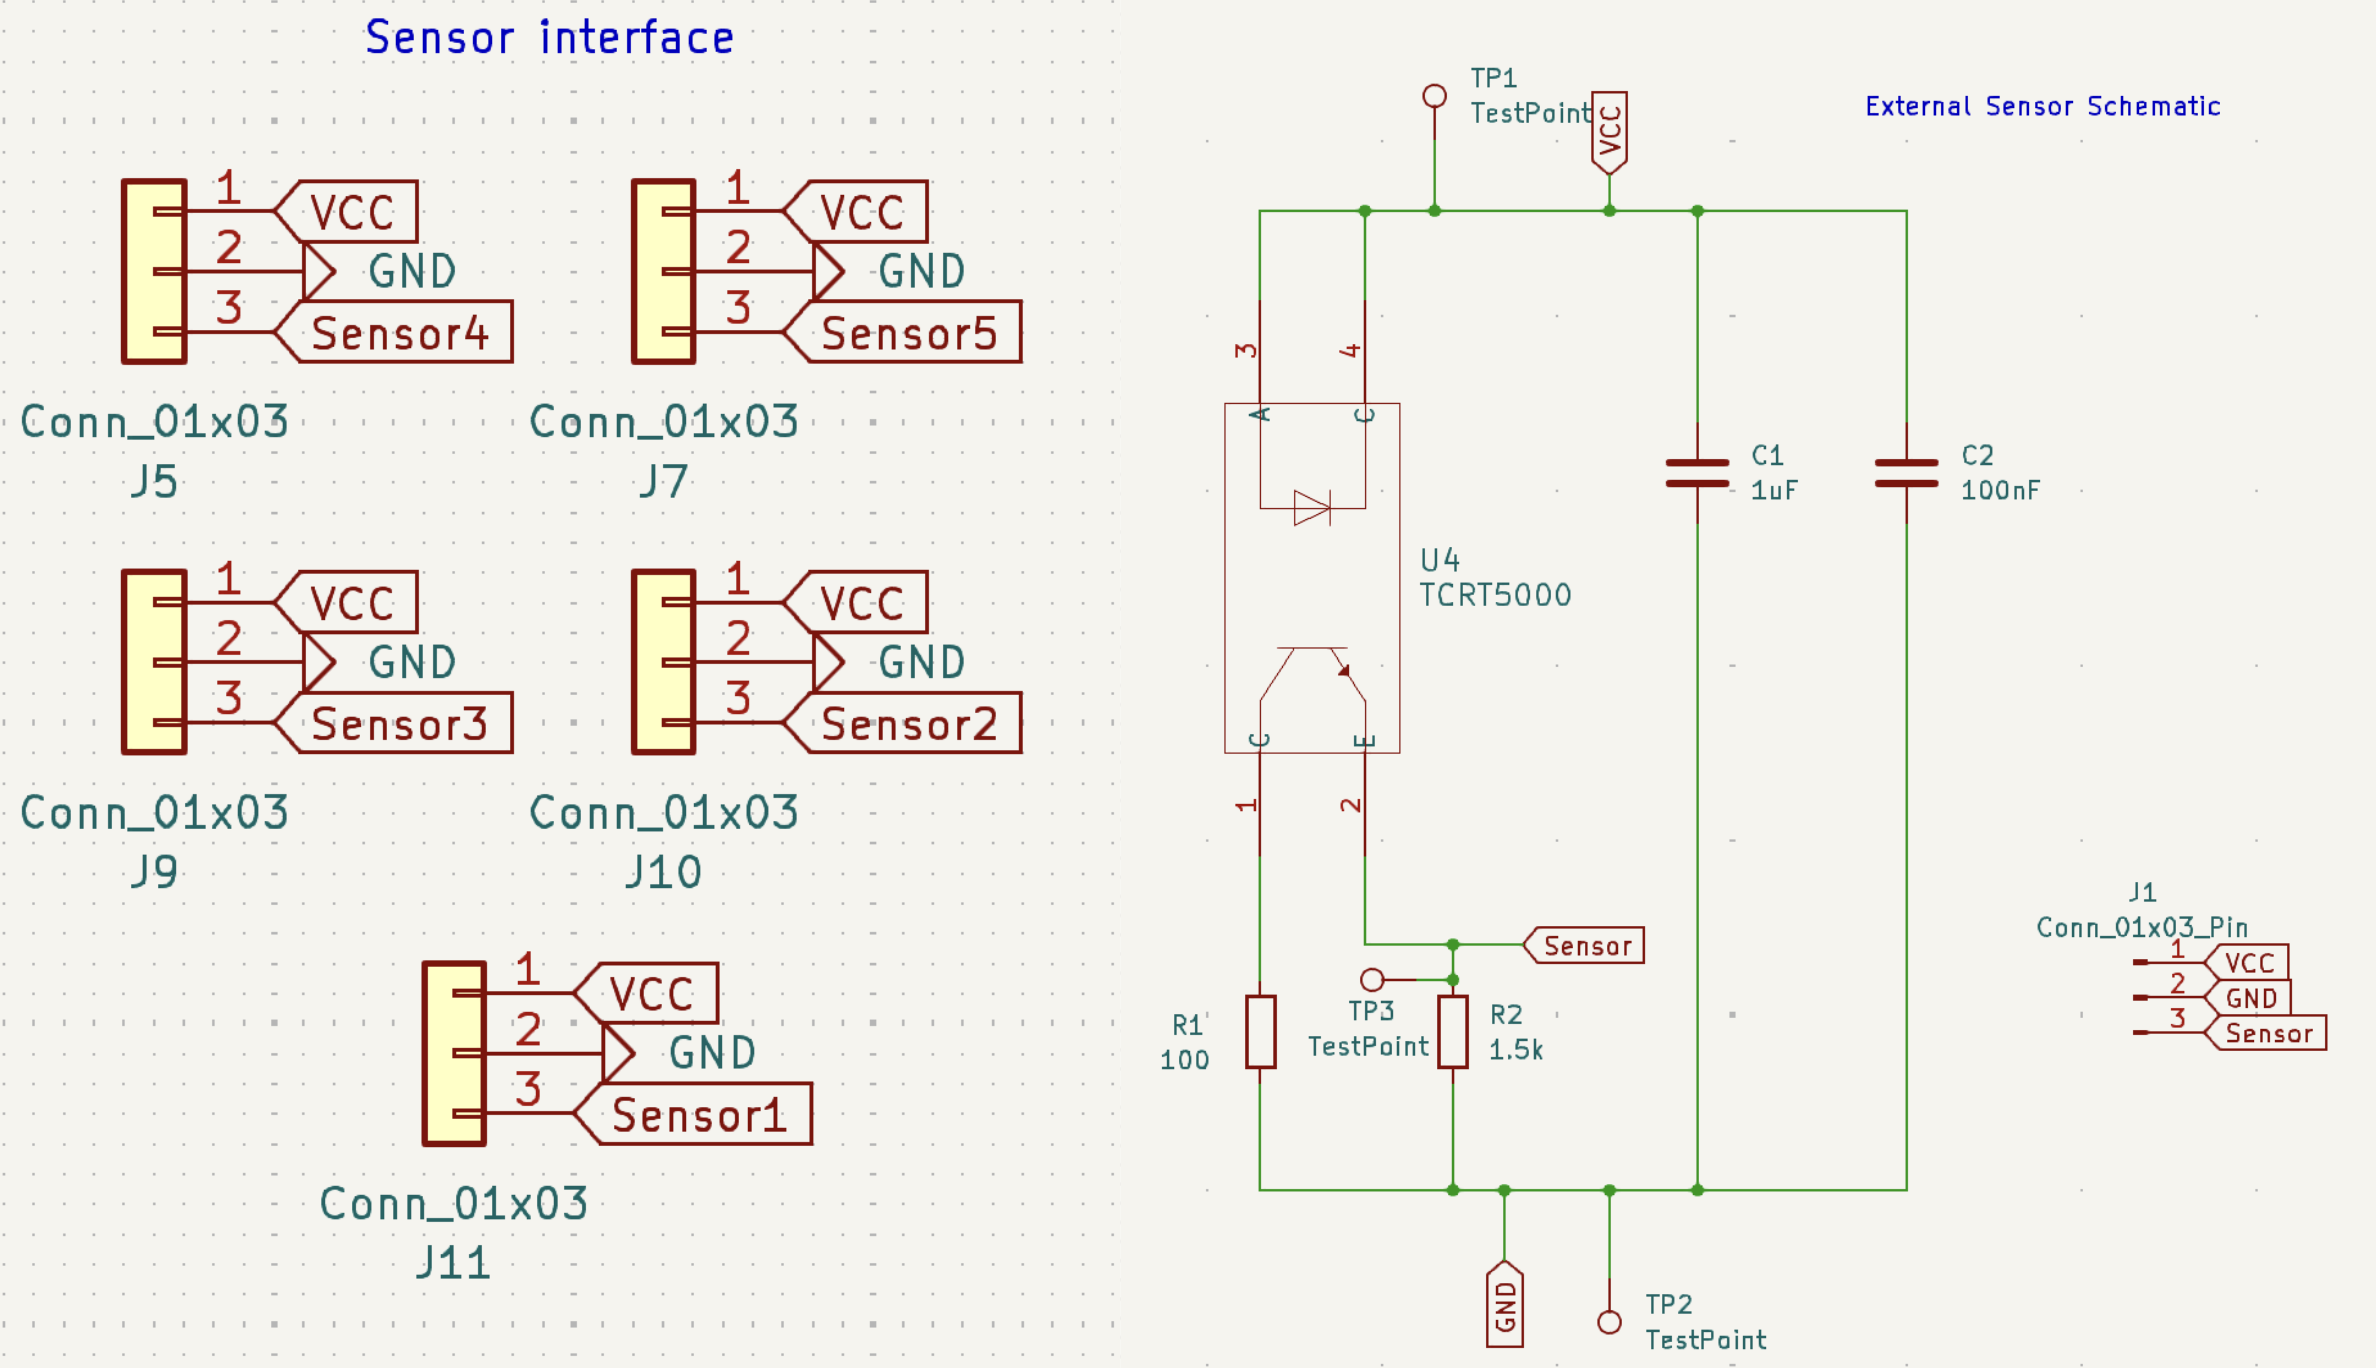
\includegraphics[width=0.7\linewidth]{REPORT/Sensor.png}
    \caption{Sensor board schematic and interface with main board}
    \label{fig:SensorSchem}
\end{figure}

The right section of Figure \ref{fig:SensorSchem} shows the schematic for the external sensor, and the left shows how it interfaces with the main PCB board. J5, 7, 9, 10 are all 3 pin connectors which have traces to VCC, GND and an input capable pin of the microcontroller, denoted by the labels Sensor1-5. These 3 pin connectors are mirrored on the sensor board with J1, allowing wires to be connected directly between the two boards. 
\\

C1 and C2 are decoupling capacitors which take out what little noise there may be from the voltage source. R1 and R2 are current-limiting resistors which prevent a short from output pins of the sensor to ground. It was discovered after the board was manufactured that this schematic was incorrect; Pins 1 and 3 should be connected to VCC, while 2 and 4 should be connected through R1 and R2, respectively, to ground. These modifications would allow current to flow through the BJT and LED inside the sensor and allow it to operate correctly. 
\\

Early in the design process, there was an idea to use an op-amp connected as a Schmitt trigger to convert the analogue output from the sensor to digital directly on the sensor board. After discussion with teaching assistants and other students, it was decided that the complications and possibilities for error of this design outweighed its benefits. 

 

\begin{figure}[H]
    \centering
    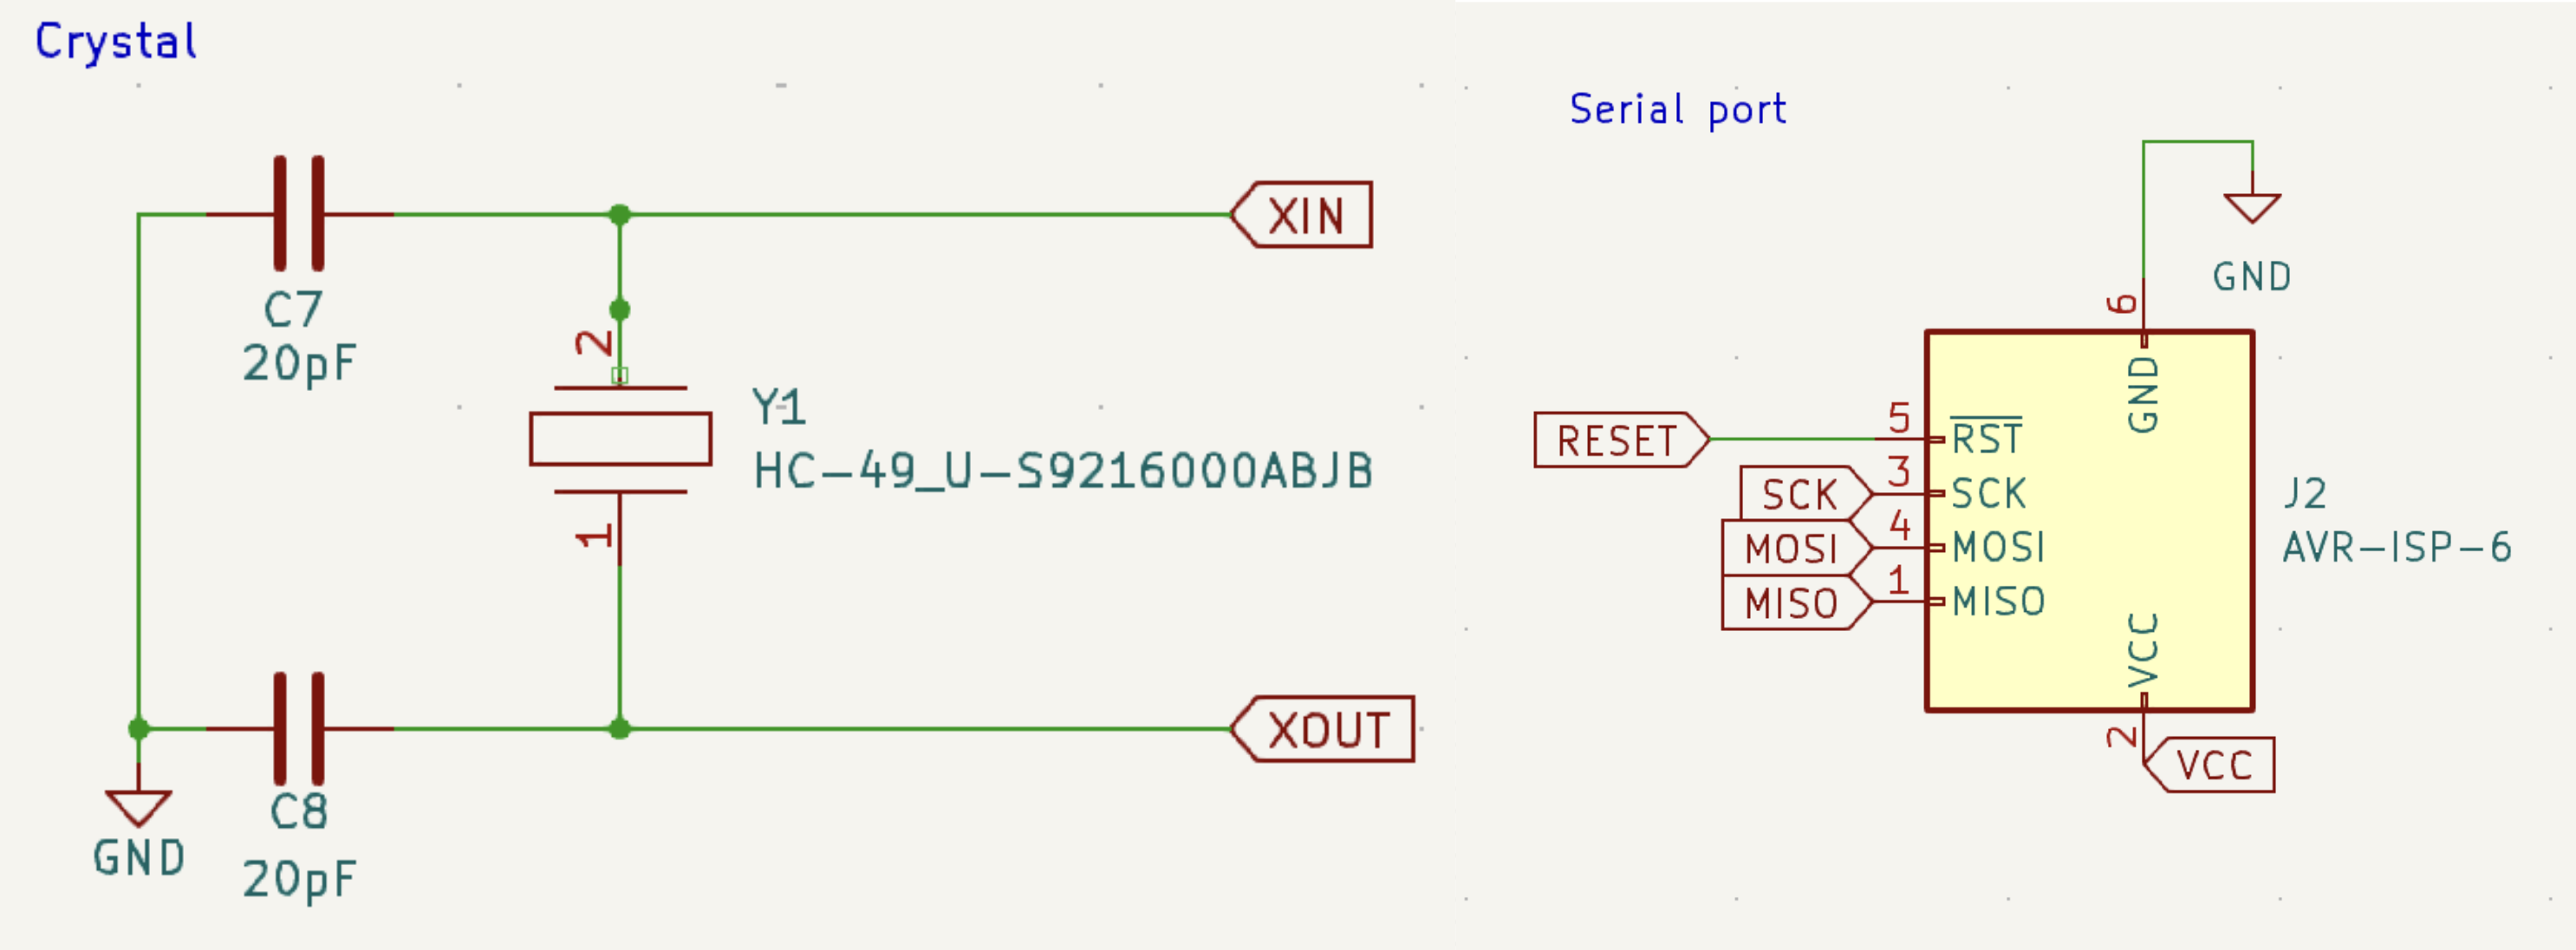
\includegraphics[width=0.7\linewidth]{REPORT/Crystal.png}
    \caption{Programming interface and crystal oscillator}
    \label{fig:Crystal}
\end{figure}

The microcontroller that was selected, the ATMEGA328, was a through-hole-mounted component. The other possibility, the ATMEGA4808, was surface-mount. As surface mount components require extreme delicacy to install correctly, it was decided that the ATMEGA328 would be used as it would ensure ease of assembly. As time constraints were one of the major considerations, this was the deciding factor. The downside of the 328 is that the internal oscillating clock used for timing operations is not ideal and is sometimes unreliable. Due to this, an external oscillating crystal was used. This is shown on the diagram as component Y1 which is connected from the XIN and XOUT pins of the microcontroller, through a set of high-frequency decoupling capacitors to ground. 
\\

The programming interface was implemented through a 6-pin connector, J2. This takes as inputs: A serial clock signal, MOSI and MISO communication channels, RESET, VCC and ground. 

\begin{figure}[H]
    \centering
    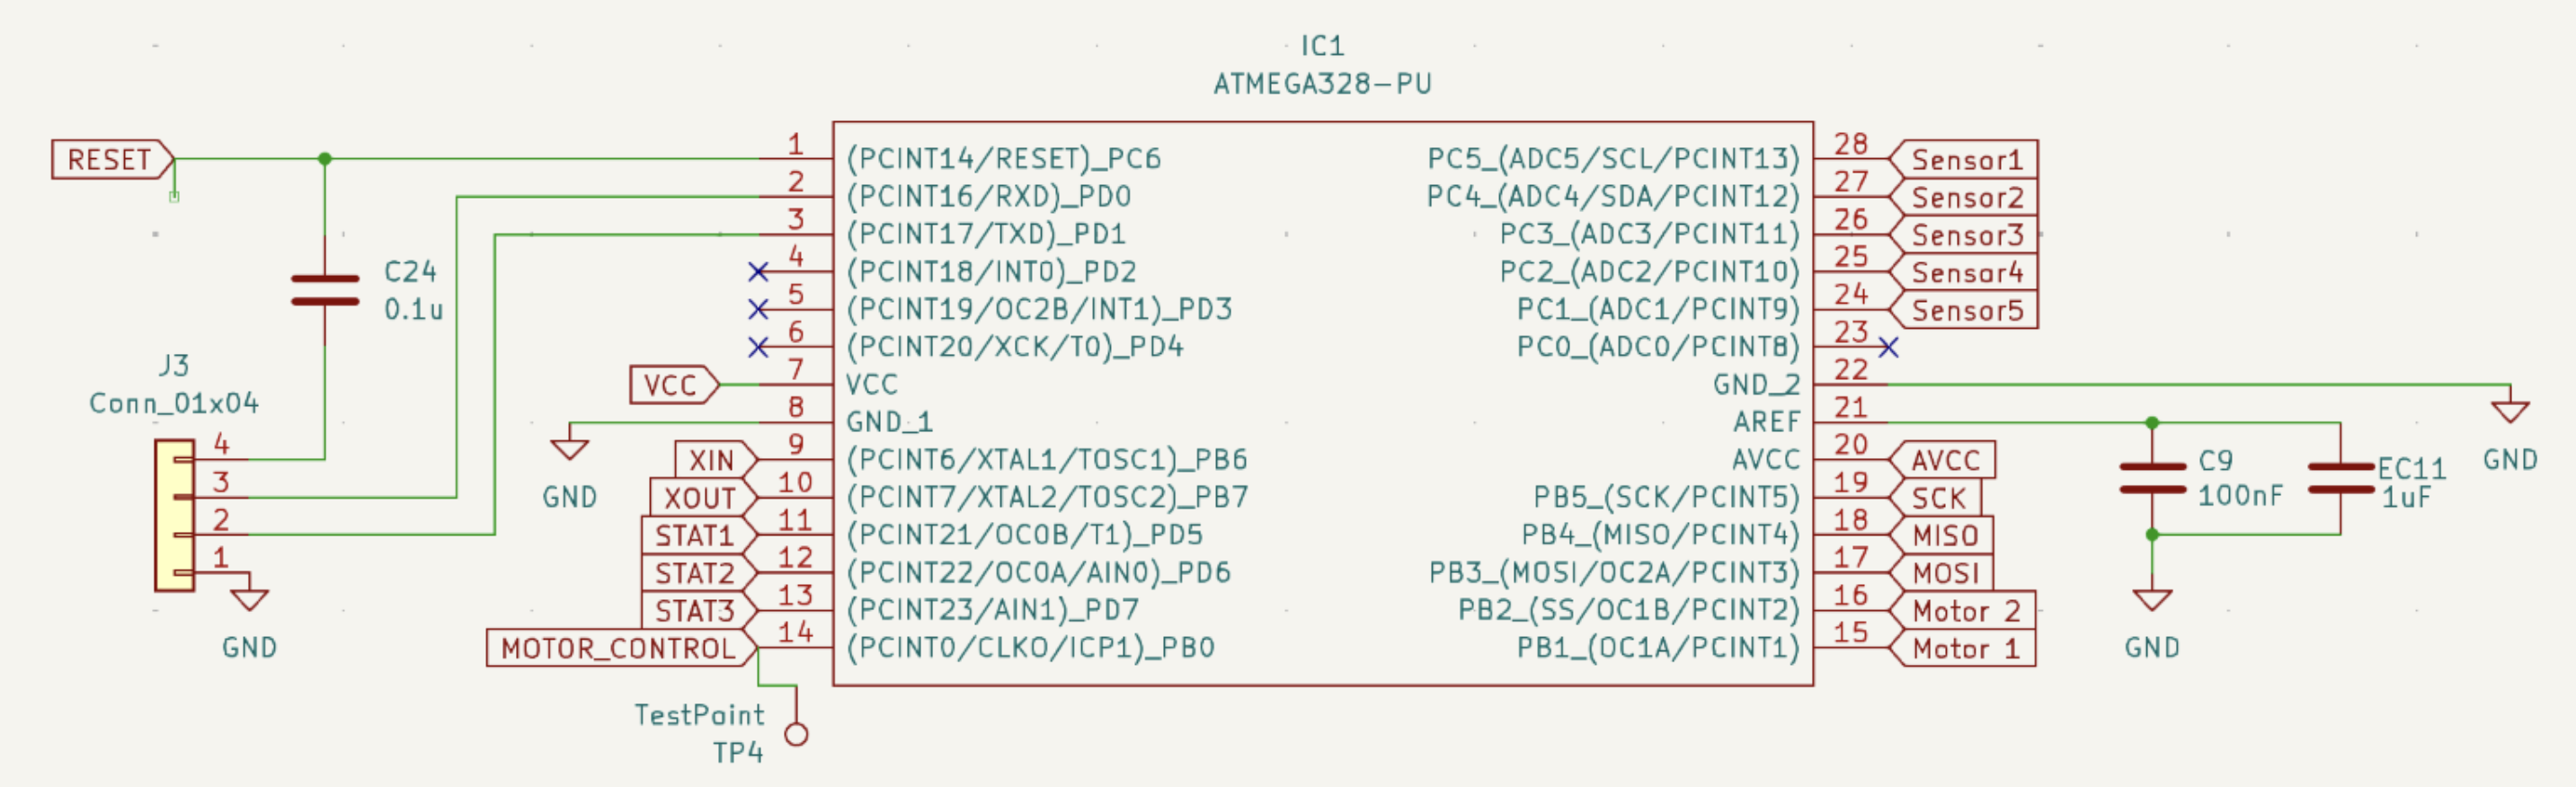
\includegraphics[width=0.83\linewidth]{REPORT/MicroCon.png}
    \caption{Microcontroller}
    \label{fig:Microcontroller}
\end{figure}

\begin{figure}[H]
    \centering
    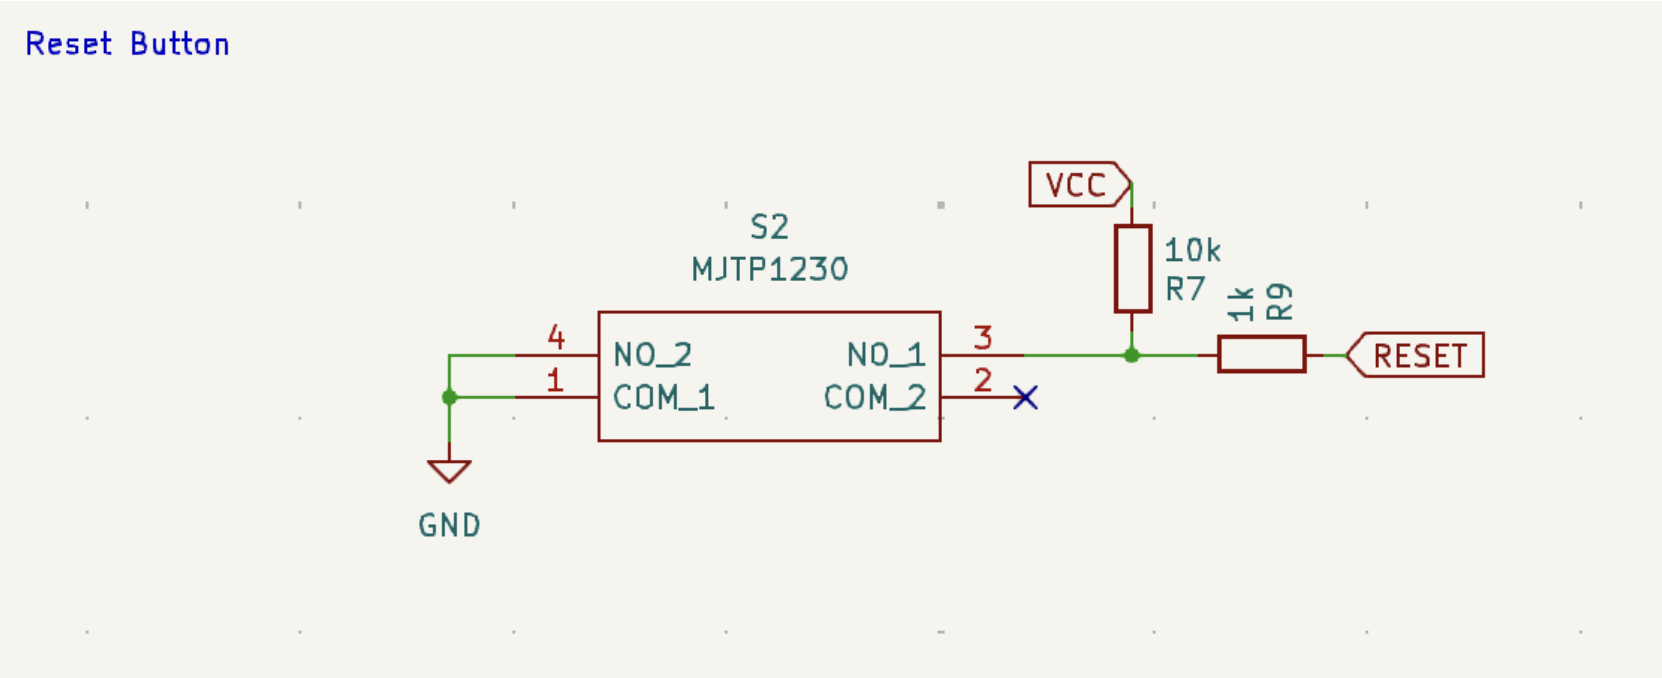
\includegraphics[width=0.5\linewidth]{REPORT/Reset.png}
    \caption{Reset button}
    \label{fig:RSET}
\end{figure}

\begin{figure}[H]
    \centering
    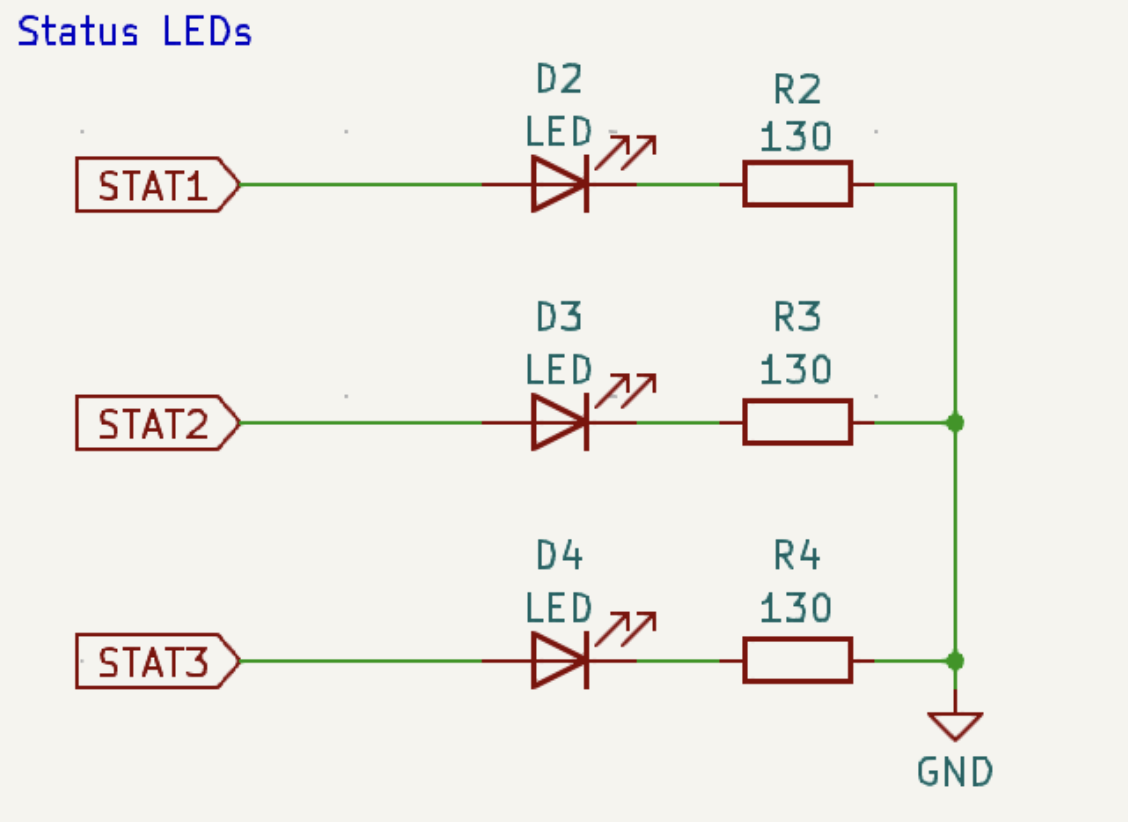
\includegraphics[width=0.35\linewidth]{REPORT/LED.png}
    \caption{Status LEDs}
    \label{fig:led}
\end{figure}

\begin{figure}[H]
    \centering
    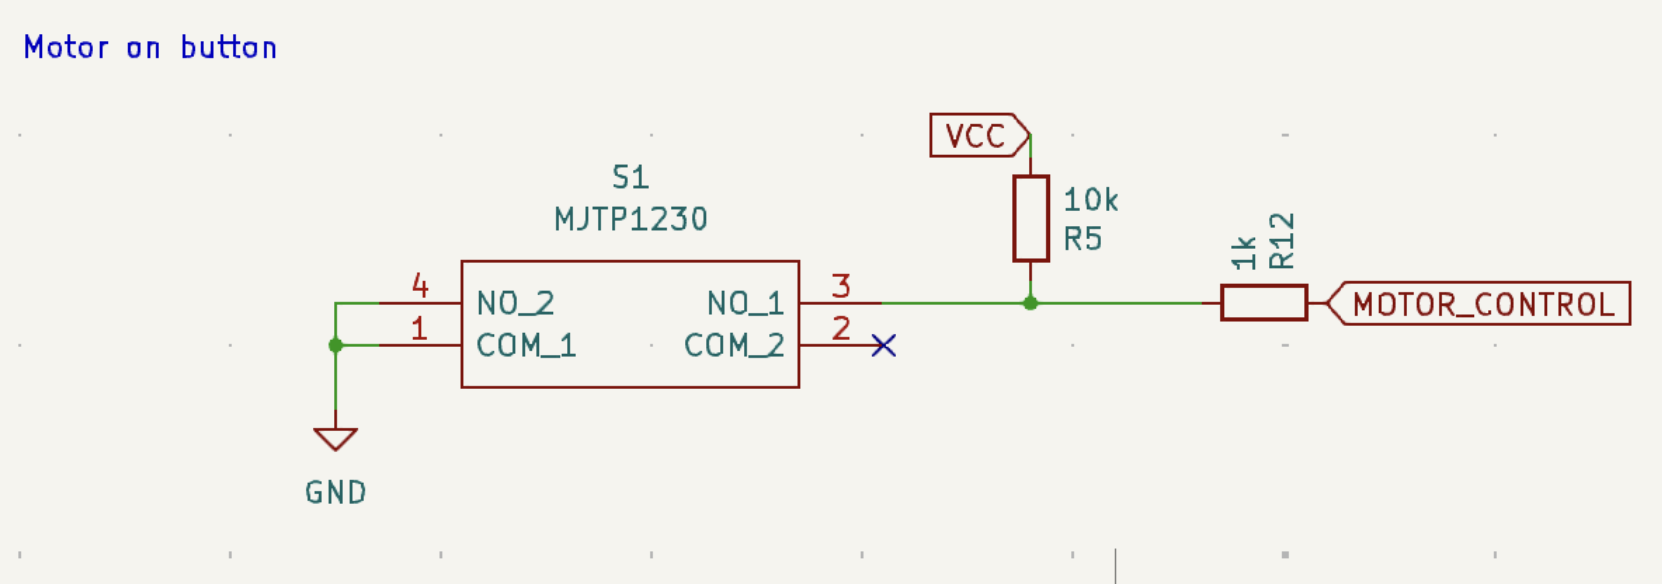
\includegraphics[width=0.6\linewidth]{REPORT/MotorON.png}
    \caption{Motor ON button}
    \label{fig:Motor ON}
\end{figure}

The two buttons - S1 and S2 in Figure \ref{fig:led} and \ref{fig:Motor ON}, were used to turn the motors on and reset the microcontroller, respectively. The VCC flag connects through resistors R7 and R5 to the input pins of the button and through R12 and R9 to ‘active low’ pins of the microcontroller. When the button is not pressed, VCC is able to flow through resistance to the microcontroller, providing it with the full 3.3V of regulated voltage. When the button is pressed, VCC is given a path to ground and shorts past the microcontroller, dropping it to 0V. At least, this is how it was designed. After assembling the board, it was found that the switches used, when pressed, connected pins 4 to 1 and 3 to 2. This meant that the voltage from VCC never had a path to ground, and thus the voltage on the microcontroller pin never dropped to 0. This issue was fixed by connecting a wire between pins 2 and 1, which allowed the button to function correctly. 
\\

The LEDs, shown in the right-hand side of Figure 5, were connected to output-capable pins of the microcontroller, enabling them to be controlled by code. As there was no way of printing outputs to check values of variables, these LEDs were invaluable in the programming stage of the project. 
\\

Finally, the microcontroller with all connected labels is shown in Figure \ref{fig:Microcontroller}. Another communication protocol (that wasn’t used) is seen in J3, which is connected to the RX and TX pins on the microcontroller, enabling a UART communication protocol.  
 
\subsection{PCB Design}
The PCB design for the main board was carried out in several stages. An initial layout (Figure \ref{fig:initpcb}) was completed to get an idea for how components might be arranged. 

\begin{figure}[H]
    \centering
    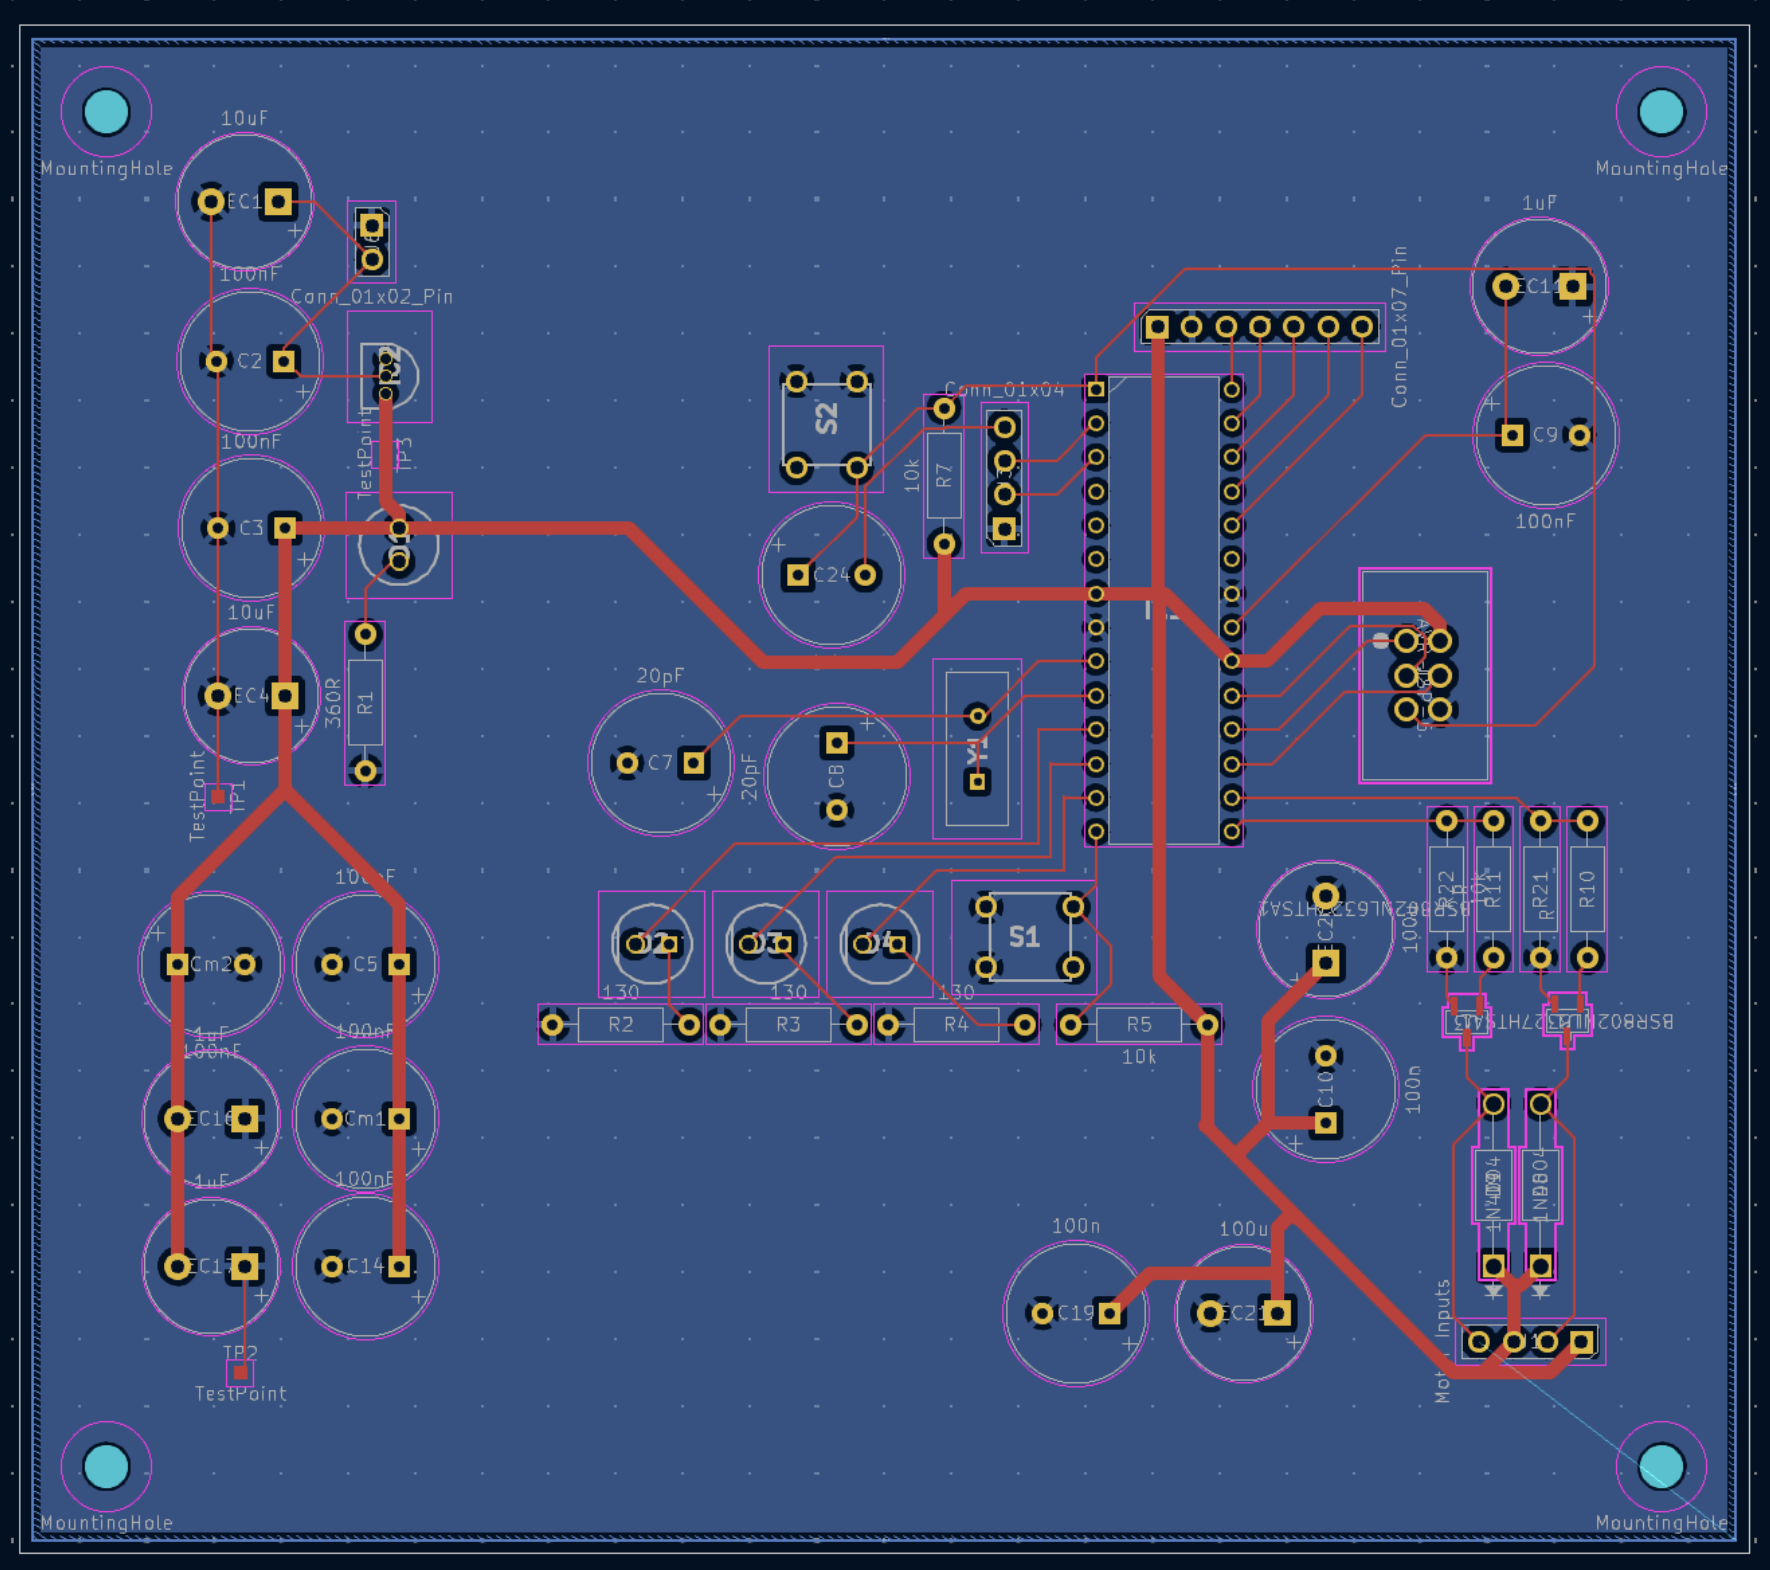
\includegraphics[width=0.4\linewidth]{REPORT/initpcb.png}
    \caption{Initial main PCB design}
    \label{fig:initpcb}
\end{figure}

The initial design took little consideration to the size of the final board. This was mostly an exercise in learning the workflow of KiCAD PCB design and was used to get feedback to complete a second, third and final iteration, which shown in Figure \ref{fig:finalpcb}. 

\begin{figure}[H]
    \centering
    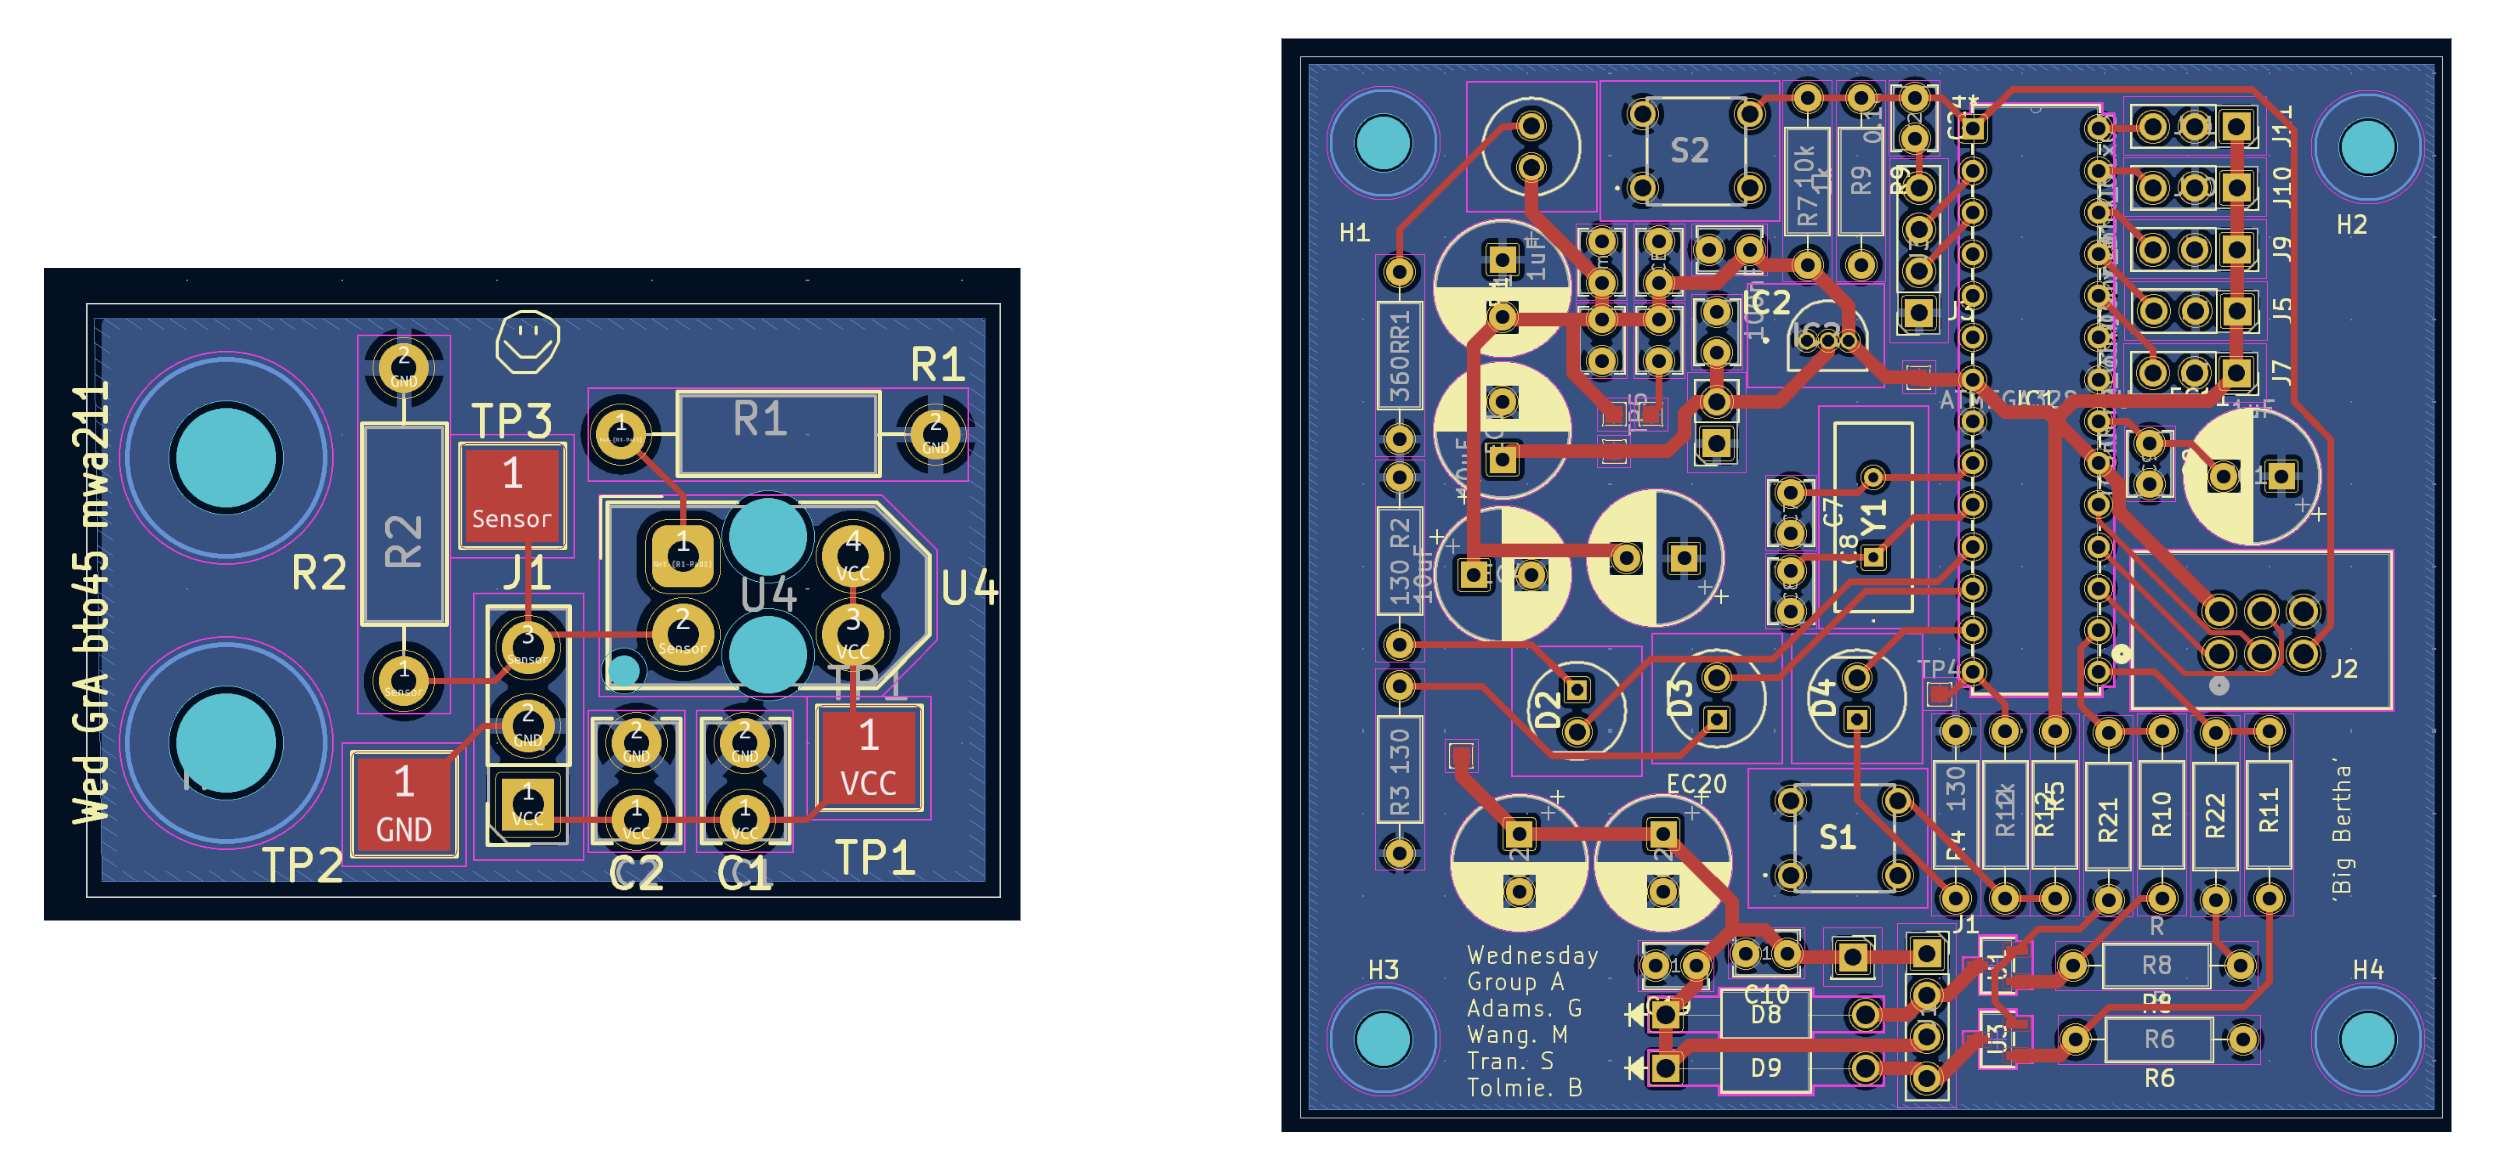
\includegraphics[width=0.7\linewidth]{REPORT/Screenshot 2024-10-20 at 2.37.22 PM.png}
    \caption{Final PCB designs}
    \label{fig:finalpcb}
\end{figure}

There were many considerations that went into the final design. The biggest of which was making traces as short as possible, which cut down on both the size of the board, and the amount of noise induced by electrical and magnetic field coupling. The second was keeping decoupling capacitors as close to the origin of their input signal as possible, to cut down on lag induced by the signal travel time and therefore increase their effectiveness. Finally, the size of the traces was considered, as higher current wires need thicker traces to ensure smooth operation. All wires carrying VCC were .8mm and larger, while all smaller signal carrying traces were left at .4mm. A few issues were encountered in selecting the incorrect footprints, as these were not provided alongside the list of allowable components. Through consultation with teaching assistants, the errors were found and corrected. 
\\

Once the design was completed, the Gerber files were extracted from KiCad and sent to JLC to be manufactured in China. This put pressure on the design process as the factory where they were being made shut down from the 1st to the $8^{th}$ of October. After some delegation and late nights, the completed boards were sent away on the $30^{th}$ of September and were received ready for assembly shortly after. 
\\

Comparatively, the sensor PCB board went through little iterations, the main changes being removing the Schmitt trigger and changing the layout to be smaller. The final design is shown alongside the main board in Figure \ref{fig:finalpcb}. 

\subsection{PCB Board Assembly}
We primarily utilised soldering irons for the PCB board assembly to solder on all the components. There are some key considerations we had to consider to ensure effective soldering.  
\\

We maintained a soldering temperature of 350 °C for all components, as this temperature allows the solder to melt quickly and adhere well to the surfaces being joined, ensuring a strong bond while minimizing excessive heat exposure. Many components, particularly sensitive electronics, can be damaged by higher temperatures, so 350 °C strikes a suitable balance by providing adequate heat for effective soldering while reducing the risk of overheating.  
\\

Additionally, this temperature promotes good flow characteristics, enabling the solder to wick into the gaps between pins and pads effectively. It also reduces the likelihood of oxidation on the surfaces being soldered, resulting in better wetting and bonding.  
\\

Since most components on our board are through-hole type, we utilized conical and chisel tips, depending on the size of the components. Like, we used a fine conical tip to minimize the risk of overheating. These tip shapes facilitate good heat transfer and allow for precision work, making detailed soldering on smaller components easier. The tapered shape of the tips enables access to tight spaces on the PCB without accidentally contacting other components, enhancing control and reducing the likelihood of soldering damage. 
\\

To ensure decent soldering quality, we also kept the soldering tip clean and tinned for efficient heat transfer, minimized the contact time to prevent damage to sensitive components like LEDs, and tested the connections with a multi-meter after soldering to ensure all the components were functioning correctly. 

\subsection{Main board adjustments}

During the testing stage, we encountered that the electrolytic capacitors were not directional which can lead to potential overheat, leakage, or even explosion due to internal pressure buildup. The polarization of these capacitors was random, which compounded the problem.  
\\

Additionally, the LED failed to turn on despite correct pin connections according to the ATMEGA328 micro-controller data sheet and the code for driving the LED. Upon a review of the main PCB layout against the schematic file, it was revealed that the issues were caused by incorrect footprints on the KiCAD PCB layout. In our case, some potential reasons could cause the incorrect footprints for the capacitors and LED. First, component rotation during the placement process may have inadvertently flipped certain components. To address this problem, we need to ensure that we check the orientation during placement and compare it with the schematic file when drawing the traces, making sure that everything is connected to the correct pin.  
\\

Second, incorrect pin mapping may have occurred if the pins on the schematic did not align correctly with the pads in the footprints. This misalignment can potentially lead to improper placement when generating the PCB layout.  
\\

Lastly, the schematic annotation may have played a role in the mismatch between the schematic and layout. It is essential to ensure that any changes made to the schematic file are promptly updated in the PCB layout to maintain consistency between the two. 
\\

Another issue that occurred in the main board assembly was the button connection, stemming from a misunderstanding of its configuration. The button features four pins, consisting of two short pins and two long pins. We incorrectly connected the button to the long pins instead of the short pins, which resulted in the button failing to complete the circuit correctly. To address this issue, we connected a wire between the long pins, so the button is now integrated into the circuit using the short pins. This way, when we press the button, it shorts to ground, allowing the circuit to function as intended. 

\subsection{Sensor board adjustments}
Figure \ref{fig:SensorAdjust} shows the layout of our sensor PCB board, along with the adjustments made based on the testing results. During the testing stage, we used a multimeter to measure the analog readings by testing the sensor pad against the ground pad. It became evident that there was no voltage drop when we covered the sensor, indicating that there was no detection of any objects. This lack of response marked the importance of precise pin connections for the TCRT500 sensor to ensure optimal functionality. 

\begin{figure}[H]
    \centering
    \includegraphics[width=0.55\linewidth]{REPORT/SensorAdjust.png}
    \caption{Sensor PCB Board layout adjustment}
    \label{fig:SensorAdjust}
\end{figure}

Upon reviewing the datasheet during the testing stage, we identified that there were some significant misconfigurations in our PCB layout. The Emitter-Cathode (pin 3 in Figure \ref{fig:SensorAdjust}) was not connected correctly with ground, impeding the current flow for the activation of the photo-transistor. To address this issue, we have made several modifications.  
\\

Firstly, we searched the traces connecting the Emitter-Cathode to the power source (VCC) and reconnected it to ground using a jumping wire. This change would allow proper current flow when the phototransistor is activated. 

Next, we scratched the traces between the Emitter-Cathode and Emitter-Anode, then connected the Emitter-Anode (pin 4 in Figure \ref{fig:SensorAdjust}) to VCC test pad with a 3.3k resistor. This modification provided a proper voltage drop and limited excessive current through the phototransistor. 

Additionally, we cut the connection between resistor R1 and the Phototransistor-Emitter (Pin 1) and reconnected the Phototransistor-Emitter to the VCC test pad using a 47 Ohms resistor. This adjustment ensures that the phototransistor is driven high when not active, facilitating correct circuit operation.  

Finally, we connected the Phototransistor-Collector (pin 2 in Figure \ref{fig:SensorAdjust}) to a pull-up resistor R2, leading to the positive voltage source. This would ensure a stable high signal when the phototransistor is off, preventing false readings.  
\\

These modifications are essential for restoring the functionality of TCRT500, ensuring the accurate detection capabilities for the Line following robot. 

\subsection{Mechanical design}
For the mechanical build, the following materials are allowed: 

\begin{itemize}  
    \item 100g of 3D printed PLA to be 3D printed.   
    \item Perspex sheet 4.5 mm thick with a bounding box of 200 × 200 mm.   
    \item M3 screws, washers, and nuts. 
    \item Rubber bands, thread. 
    \item Purely decorative elements. 
    \item Multicomp MM10 DC motor.
    \item Multicomp MM28 DC motor.
\end{itemize}  
The robot is fully printed from PLA using Bambu 3D printers from the University of Canterbury Mechanical Engineering Department. This method allows for rapid ideation and prototyping, allowing the design to be fine-tuned throughout the project.  

\subsubsection{Main Body}
The main body must serve as a base to attach the main PCB, sensor PCB modules, battery packs, wheels, and motor hinges. Initially, the main body was planned to be laser cut from an A3 Perspex acrylic sheet so that the 100g of printed PLA can be allocated to solely the wheels and motor hinges. The weight limit, however, was not an issue, and PLA was used for the main body as it allowed for decorative details and rapid prototyping (access to 3D printing is 24/7).  
\\

As shown in Figure \ref{fig:MainBod}, the initial design intended to have a raised platform for the PCB, housing the power source underneath. After printing and testing this, it was discovered that the power source is better mounted on the underside of the body, leaving much more room on top. This is more optimal as it maintains the proximity of the batteries to the PCB, reducing the risk of stray inductance/noise in the circuit, as well as lowering the centre of mass which increases the efficiency of the dynamics. 
\\

The final design also included a lot more 3M holes. This decreased the mass of the robot, but more importantly, it allowed more customisation and flexibility during the latter stages when the robot was being assembled and tested.  

\begin{figure}[H]
    \centering
    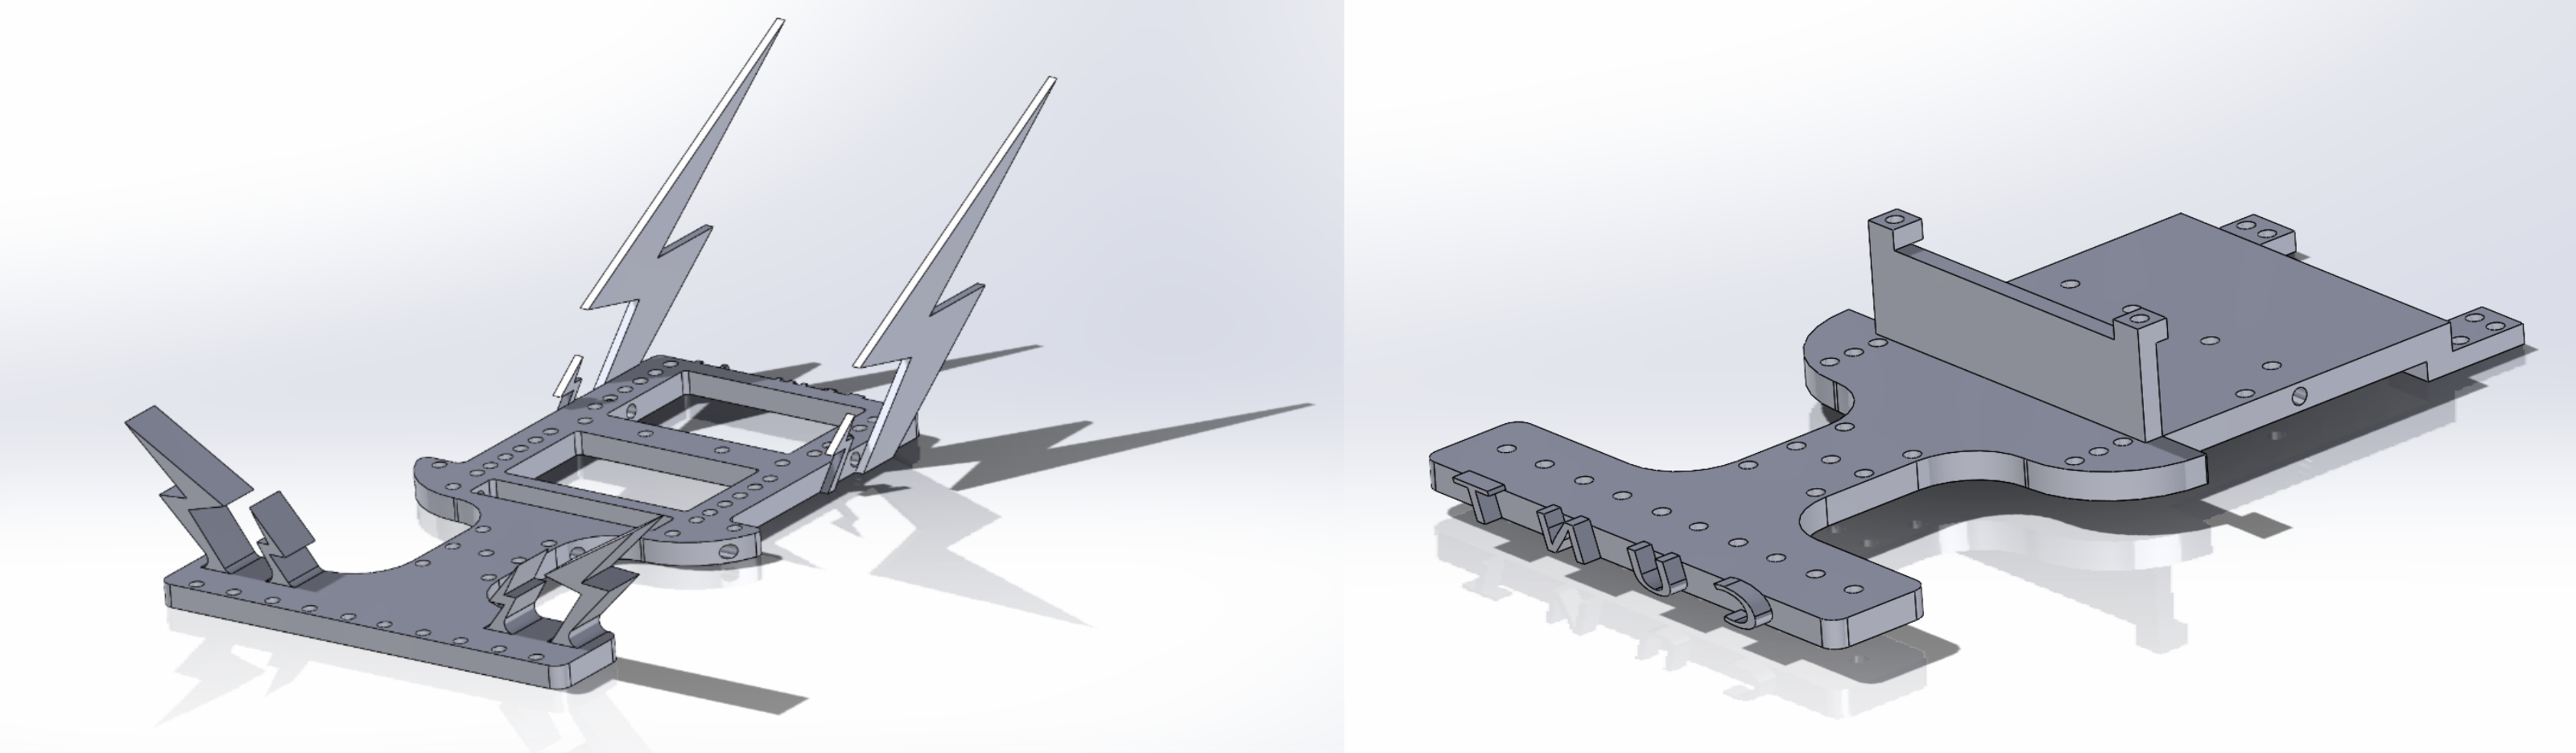
\includegraphics[width=0.7\linewidth]{REPORT/MainBod.png}
    \caption{Main body isometric view – Final vs. Initial design}
    \label{fig:MainBod}
\end{figure}

\subsubsection{Motor hinge}
The motor hinge design was kept basic as shown in Figure \ref{fig:Motorhinge}, with the motor holding being 0.1mm larger than the motor diameter dimension to create a transition fit that tightly holds the motor in place. To keep the motor from sliding out, the bottom was dimensioned 1mm smaller, this ensured stability yet easy access to the wiring pins. Lightning bolt extrusions were added to match the aesthetic theme of the main body. The motors spin the wheels via direct contact drive, so the lightning bolts also served as a ledge to hold a counterweight we implemented in the final design. This counterweight was made from our prototype wheels as a casing, and broken DC motors as weights; this reduced wasted material. 

\begin{figure}[H]
    \centering
    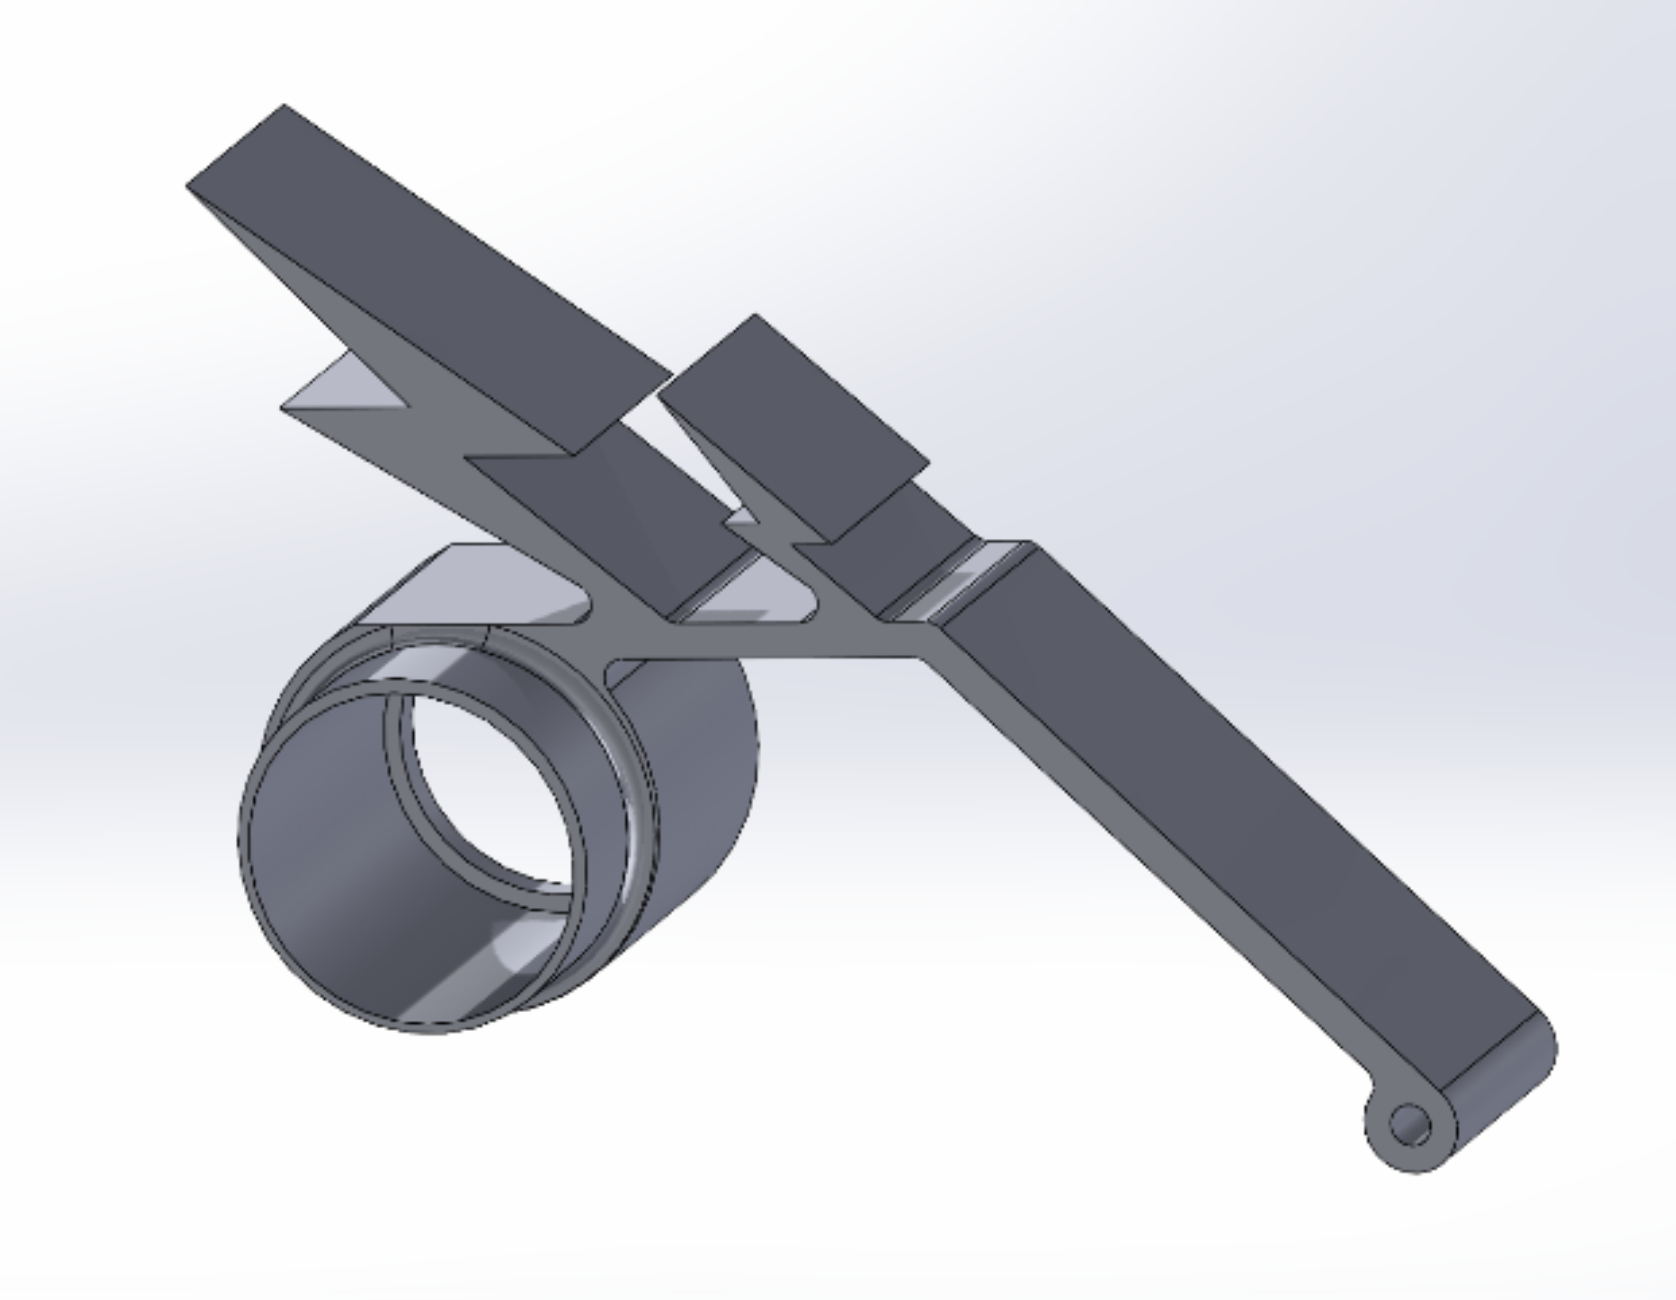
\includegraphics[width=0.3\linewidth]{REPORT/MotorHinge.png}
    \caption{Motor Hinge isometric view}
    \label{fig:Motorhinge}
\end{figure}

\subsubsection{Wheels}
Two variations of the wheel design were manufactured, thin and thick as shown on the left and right of Figure \ref{fig:Wheels} respectively. 50, 55, 60, 65, and 70mm diameter dimensions were trialled throughout the project. The final wheel on the robot was a 55mm thick wheel. The smaller diameter had a smaller moment of inertia, which required less torque to rotate whilst still being large enough so that the motor hinges did not interfere with the electronic components of the main PCB. 

\begin{figure}[H]
    \centering
    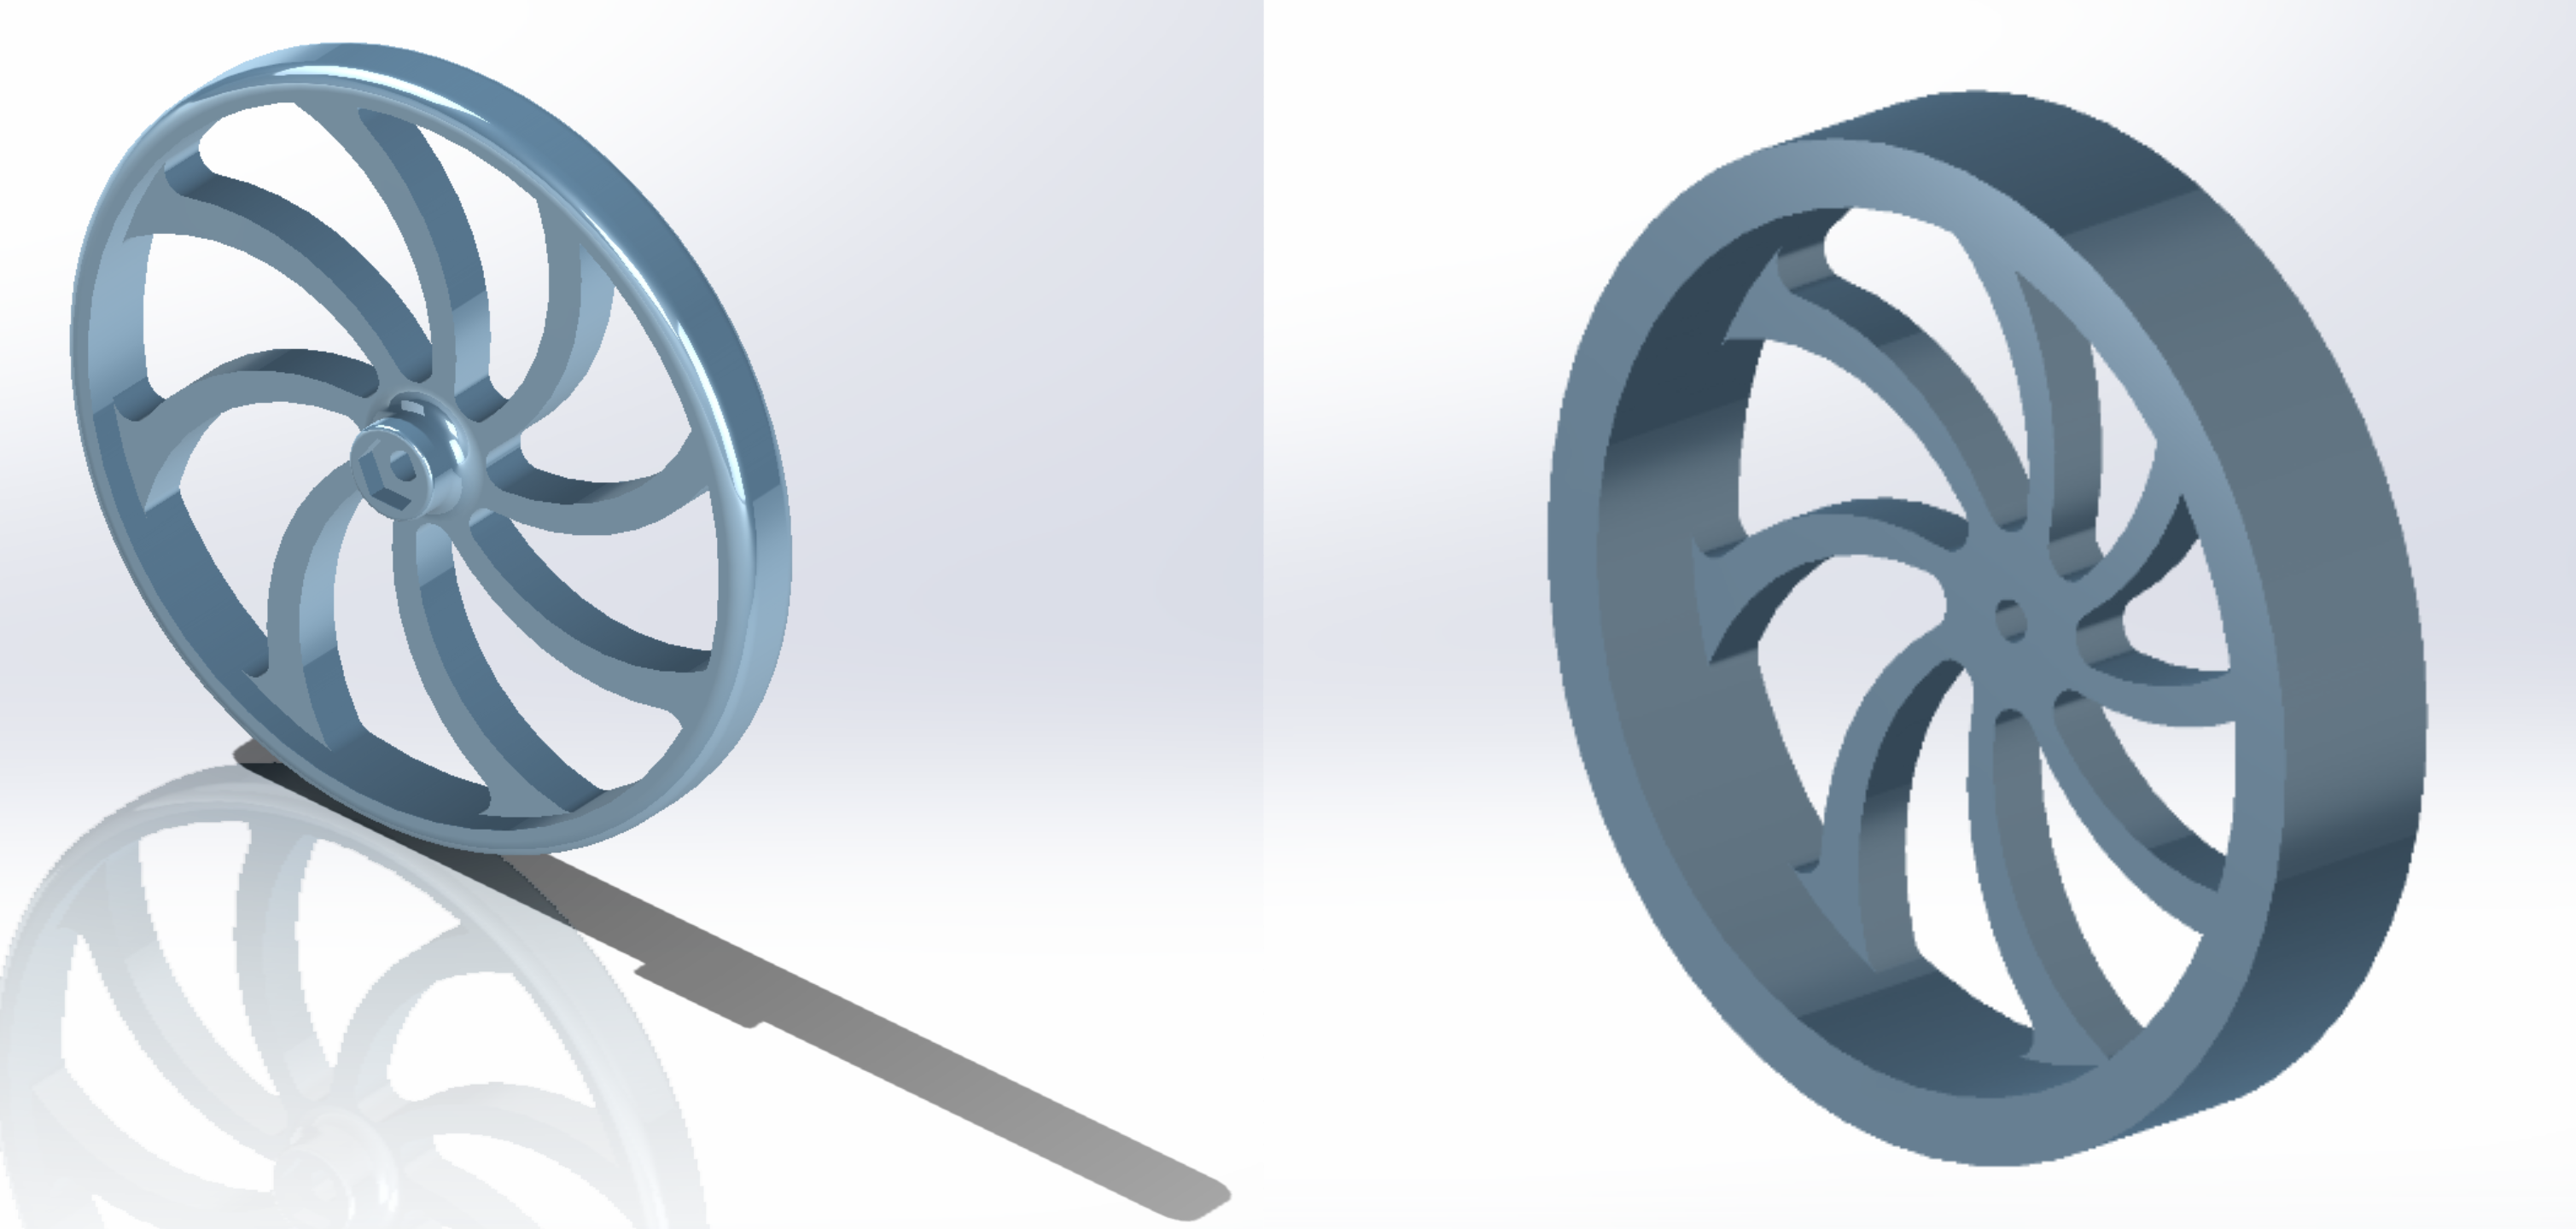
\includegraphics[width=0.5\linewidth]{REPORT/Wheels.png}
    \caption{Thick and thin wheel design variations isometric view}
    \label{fig:Wheels}
\end{figure}

\subsection{Software}
A reactive controller was made using Arduino programming, code in Appendix A. The reactive control depended on the immediate feedback of 3 sensors, left, centre, and right, where each sensor was compared against a threshold value to detect if the sensor was on the line. The robot was placed with the line central to the centre sensor. The robot would turn left if the right sensor detected the line, right if the left sensor detected the line, and forward if the centre sensor detected the line. This closed-loop control system minimized the error of the distance from the line, providing a simple, robust and responsive method of following the line.  

\section{Results \& Discussion}
The software part of the line-following-robot started with high expectations of a working PID controller. However, our sensor boards had issues so only 2 sensor boards worked during the programming phase. This made PID control overly complex for our robot, so a reactive controller was made using Arduino programming, code in Appendix A. A limitation to having feedback from 2 sensors was the oscillations of the robot due to the sensors continuously triggering changes in direction without settling. This reduced the potential top speed of the robot. 
\\

To combat this, a third sensor positioned at the centre was added, and the robot moving forward when the sensor detected the line. By adding a third sensor, there was an average 4.9-second increase in course performance times, outlined in the ‘Course Times by Sensor Configurations and Weight’ table in Appendix B. This time saving was expected due to increased feedback allowing the sensors to occasionally settle in a forward state when the centre sensor detects the line. In doing so, the robot followed the line more smoothly, allowing for increased speeds. Therefore, to further reduce the average course time from a software perspective, a working PID and more sensors closely spaced together would be recommended. Weight was added to above the motors to increase the friction between the motors and wheels. Rough blotches of solder were also melted onto the motor shafts, which allowed it to grip the wheels better. Figure \ref{fig:Trialchart} shows the results of these optimisation changes. 

\begin{figure}[H]
    \centering
    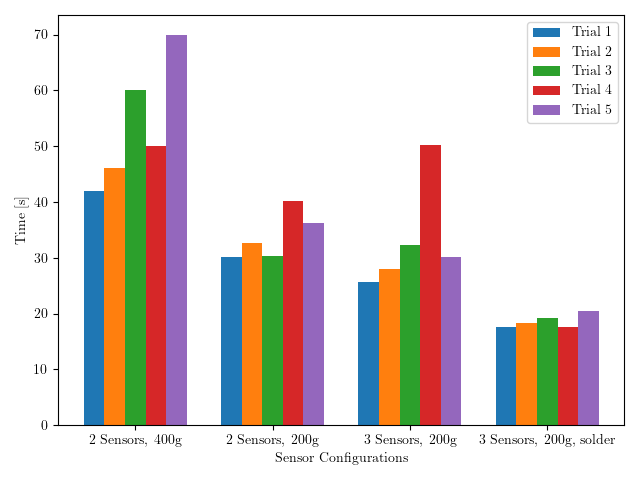
\includegraphics[width=0.5\linewidth]{REPORT/plotv3.png}
    \caption{Line Following Robot Course Times by Sensor Configurations and Weight }
    \label{fig:Trialchart}
\end{figure}

The Line Following Robot performed competitively well in the final demonstration, finishing the course in 14.939 seconds on our first attempt. A video of the robot's final run can be accessed with the following link: \href{https://youtu.be/P_ezBJ8gyDk}{$https://youtu.be/P_ezBJ8gyDk$}. The robot tracked the line reasonably accurately, with only minor overshooting when trying to make turns, which was within an acceptable range. After the first trial, we attempted to move the sensors closer together to improve line detection accuracy and reduce overshooting, thereby increasing speed. However, this approach failed during testing due to interference between the sensors when they were positioned too close to each other. 
\\

Our second solution was to gradually increase the forward speed of the robot. However, this caused other issues, such as difficulty in maintaining accurate line detection, which led to increased deviations from the path and potential loss of control. The robot struggled to respond quickly enough to changes in the line’s direction, resulting in more frequent overshooting of turns and ultimately decreasing its overall performance and reliability in navigating the course. We tried several speed settings but couldn’t achieve a result better than our first trial. Due to time pressure, we were unable to conduct another trial. 
\\

Looking ahead, several solutions could yield better results. First, we could program an additional sensor, allowing the robot to utilize four sensors for improved line tracking and reduced overshooting. Secondly, we were using bang-bang control, which only has two states, on or off based on whether the robot is on or off the line. Transitioning to a PID control system could enhance performance. Proportional control would respond to the current error (the difference between the desired position, centred on the line, and the current position), integral control would address the accumulation of past errors to eliminate steady-state error, and derivative control would predict future errors based on the rate of change, helping to dampen the system and reduce oscillations. This approach could allow our robot to increase speed while following the line more accurately and with less overshooting during turns. 
\\

Moving forward from this project, we have gained a better understanding of the importance of real-world testing. If this project were to be repeated, we would allocate more time toward improving the design of the PCB board and conducting thorough software testing. 

\section{Conclusion}
 The Line Following Robot project involved circuit design, PCB layout, mechanical assembly, and control systems. While we encountered challenges, particularly with sensor board malfunctions and feedback control, the robot still performed well, completing the course in 14.939 seconds. By using a reactive control system, we were able to achieve consistent results, though transitioning to a PID control system could improve accuracy and make the robot’s movements smoother. This project emphasized the importance of testing and collaboration to work through design unpredicted errors. Moving forward, further improvements could be made by refining sensor placement, improving the control system, and optimizing the mechanical design. Overall, the project met its objectives and gave us practical experience in combining different areas of mechatronics engineering.

\newpage
\bibliographystyle{ieeetr}  % The style of the bibliography (e.g., plain, alpha, etc.) 
\bibliography{references}

\newpage
\appendix
\section{Arduino Code for Line Following Robot}
\subsection{Overview}
The code was programmed using Arduino. Only the .ino, .cpp and config.h files are included in Appendix B. For full code including .h files, access the GitHub: \href{https://github.com/blaketolmie/LFR}{https://github.com/blaketolmie/LFR}
\subsection{LFR\_Main.ino}

\begin{figure}[H]
    \centering
    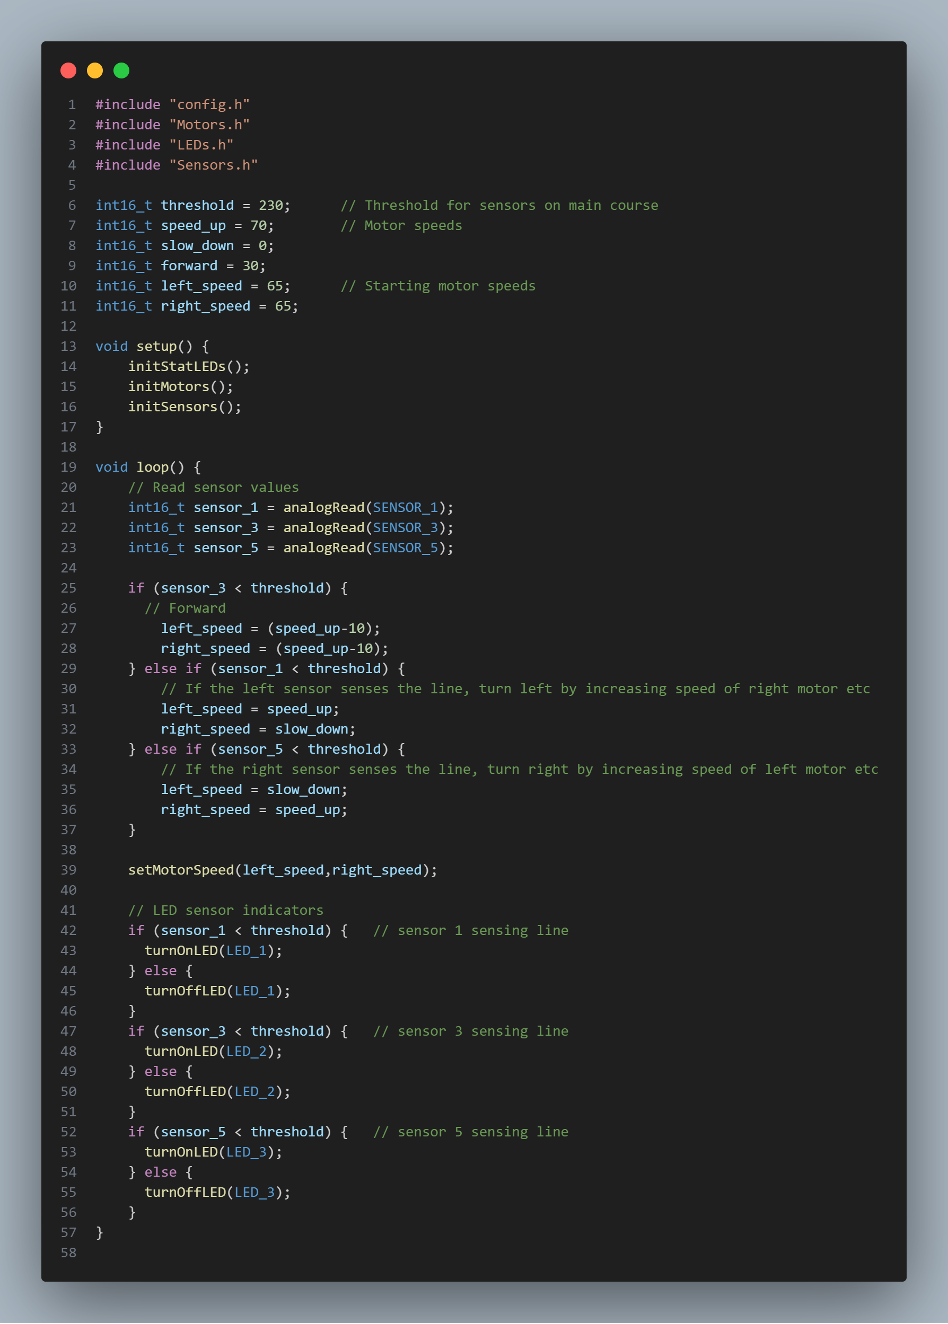
\includegraphics[width=0.8\linewidth]{REPORT/LFR_main.png}
\end{figure}

\subsection{Motors.cpp}

\begin{figure}[H]
    \centering
    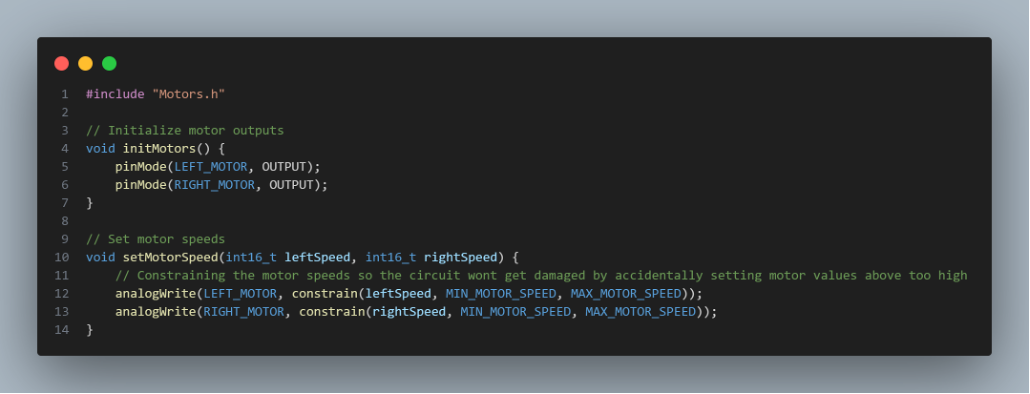
\includegraphics[width=0.8\linewidth]{REPORT/Motorscode.png}
\end{figure}

\subsection{Sensors.cpp}

\begin{figure}[H]
    \centering
    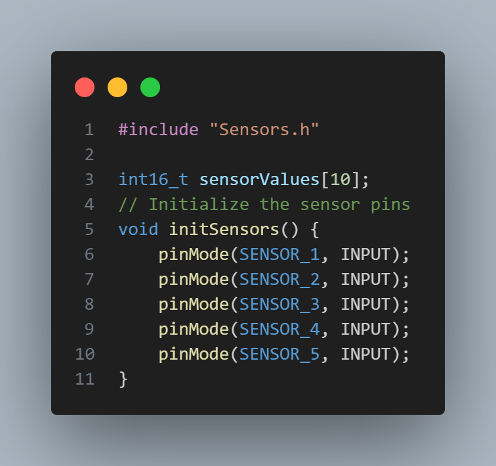
\includegraphics[width=0.8\linewidth]{REPORT/sensorscode.png}
\end{figure}

\subsection{LEDs.cpp}

\begin{figure}[H]
    \centering
    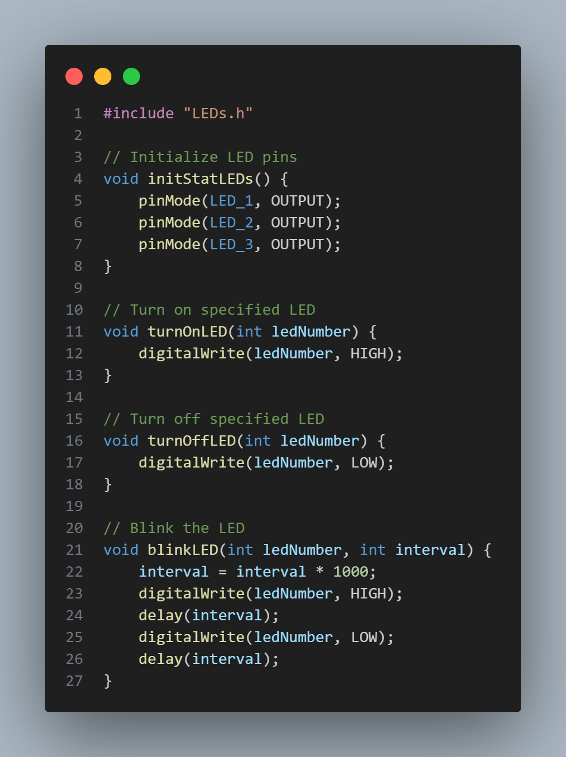
\includegraphics[width=0.8\linewidth]{REPORT/ledscode.png}
\end{figure}

\subsection{Config.h}

\begin{figure}[H]
    \centering
    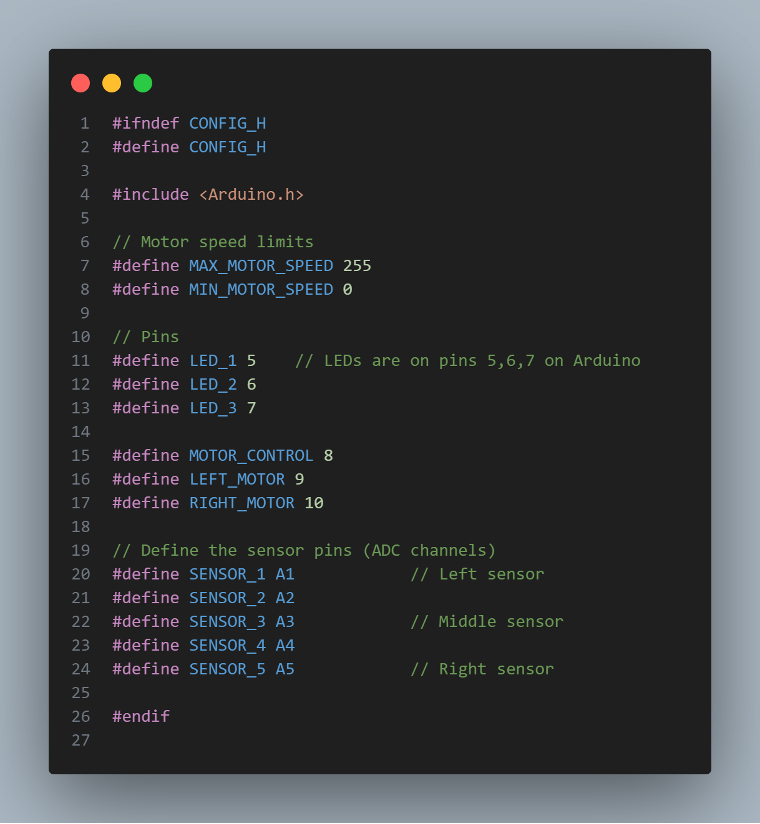
\includegraphics[width=0.8\linewidth]{REPORT/configcode.png}
\end{figure}

\section{Table for LFR Course Times by Sensor Configurations and Weight}
\begin{figure}[H]
    \centering
    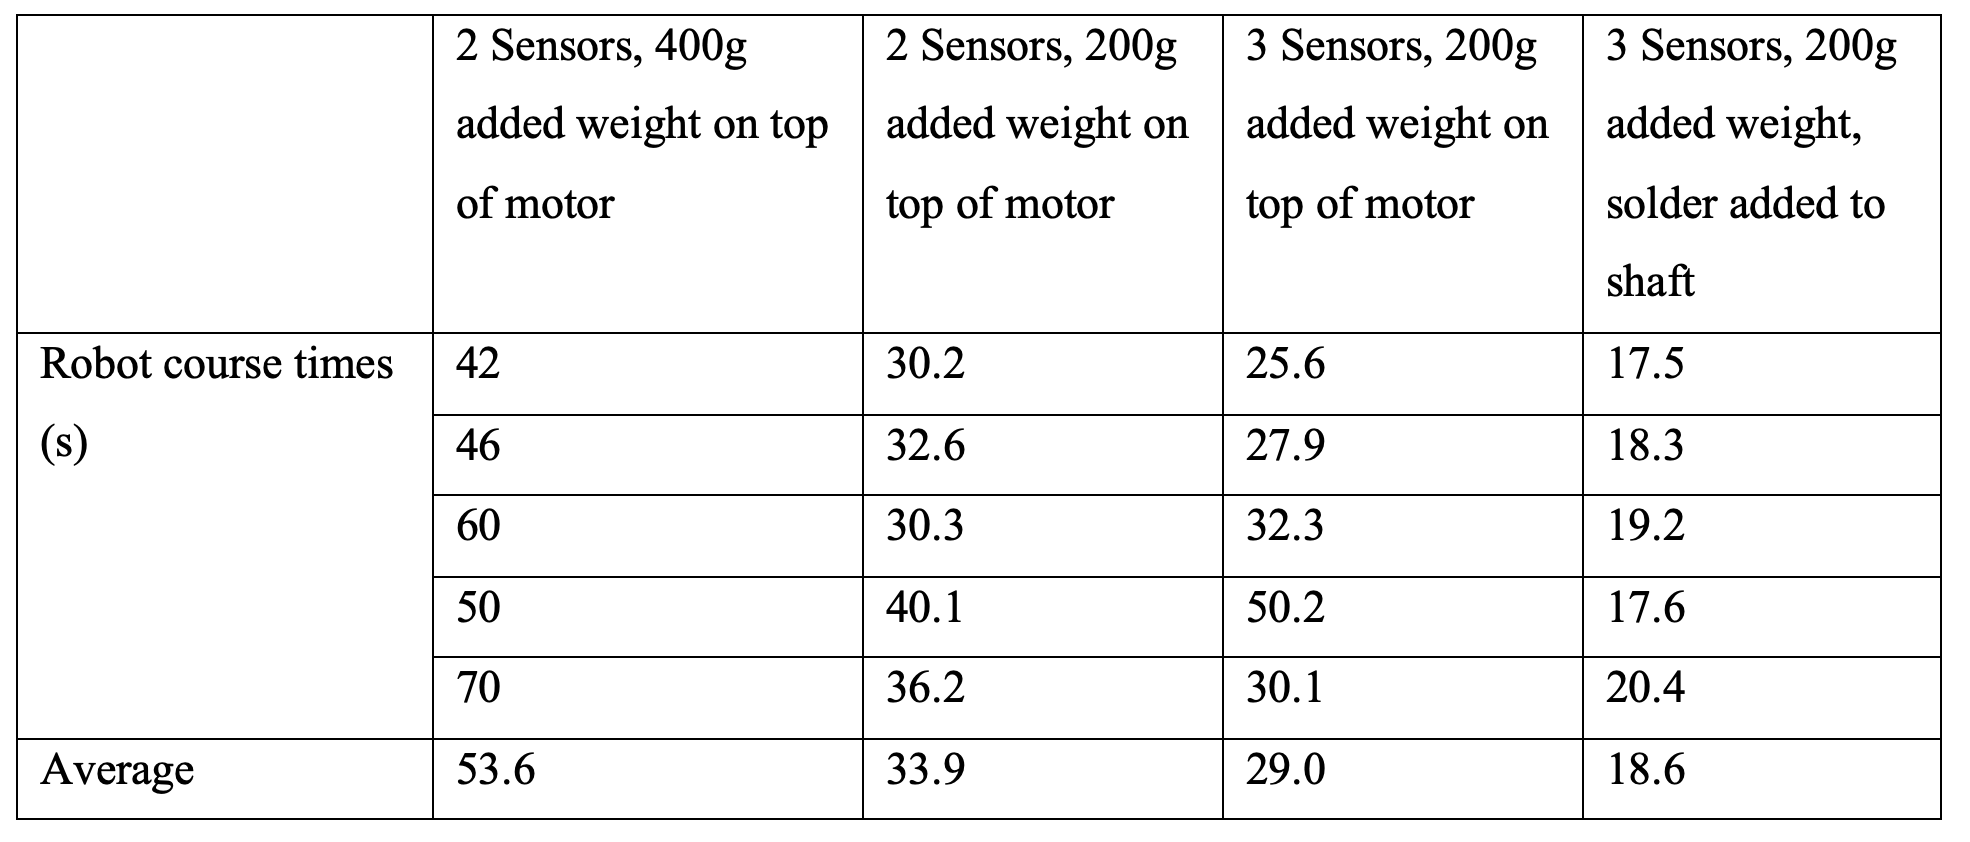
\includegraphics[width=0.8\linewidth]{REPORT/Screenshot 2024-10-20 at 3.11.46 AM.png}
\end{figure}

\section{Allowed Electronic Components}
\begin{figure}[H]
    \centering
    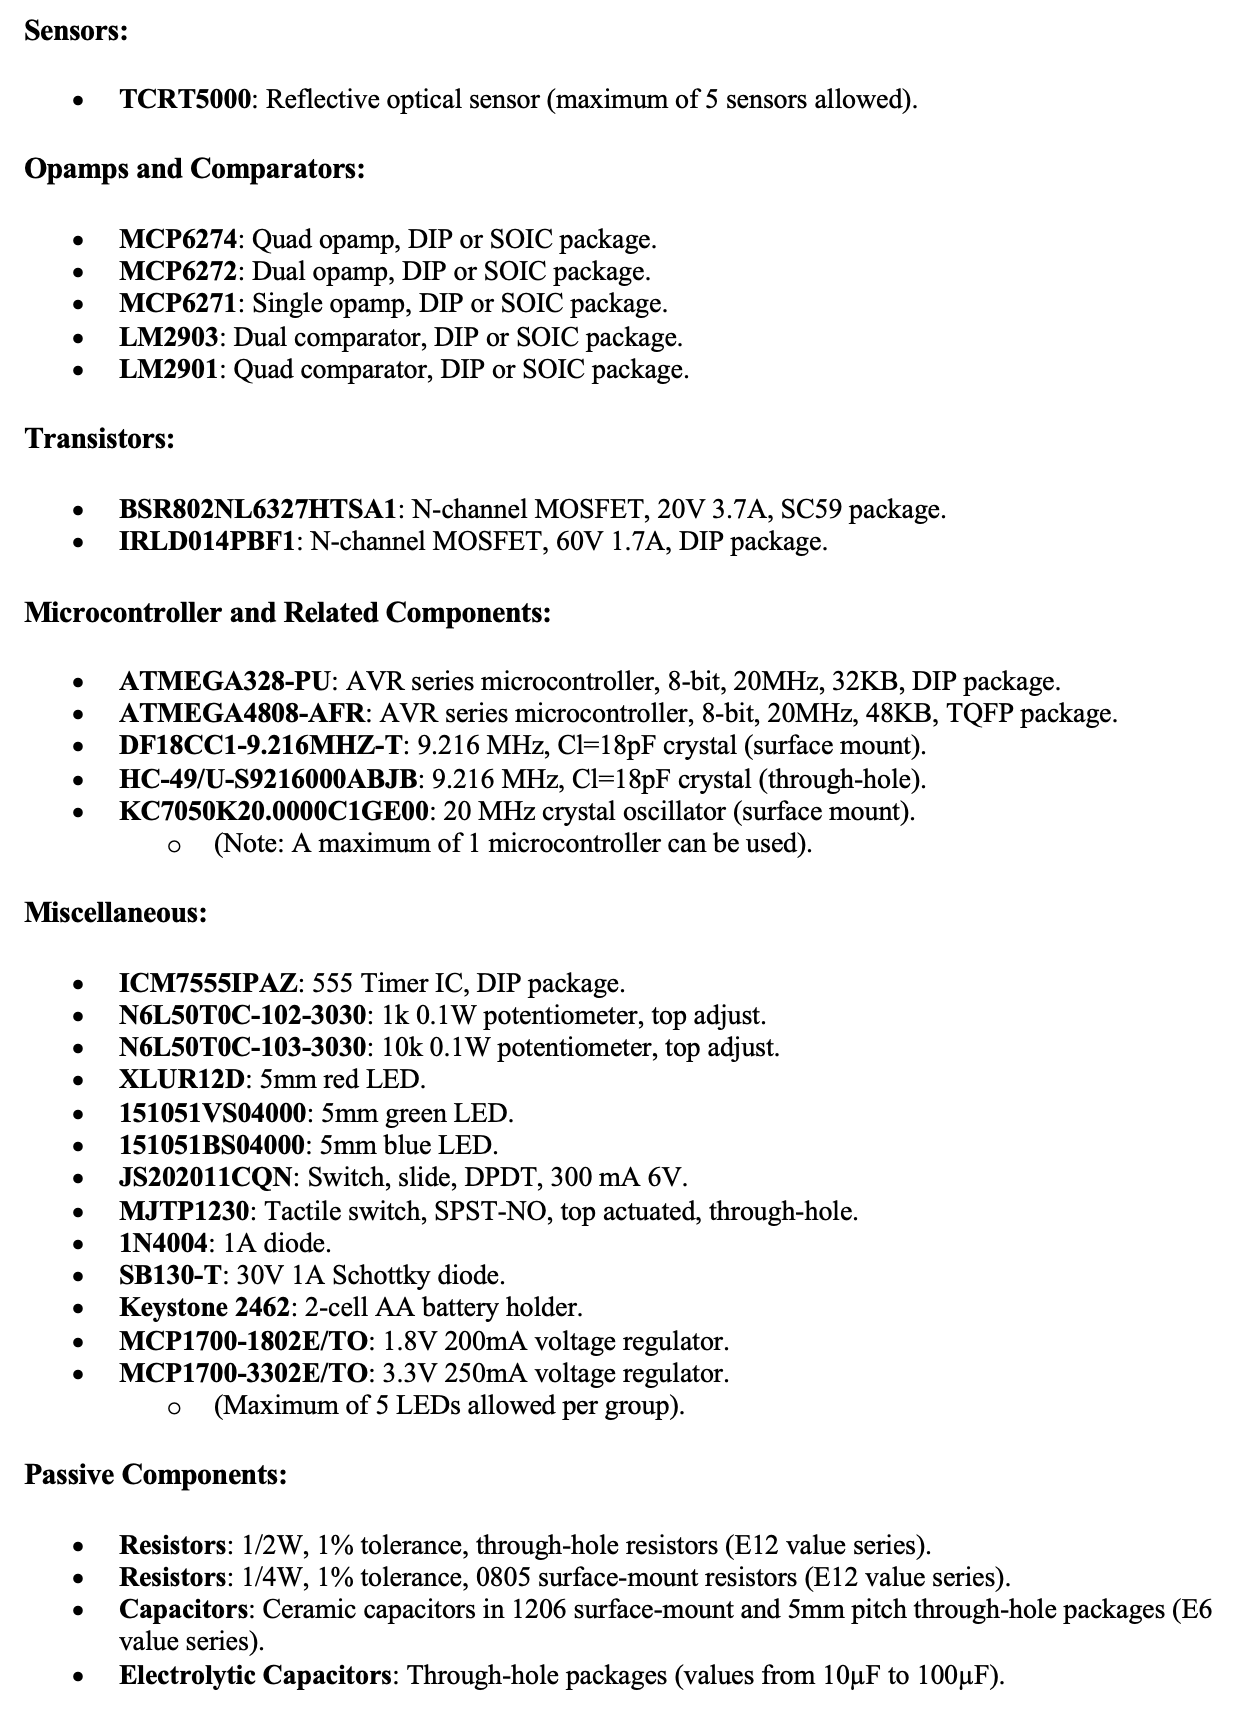
\includegraphics[width=0.8\linewidth]{REPORT/Screenshot 2024-10-20 at 3.10.45 PM.png}
\end{figure}

\end{document}